\documentclass[10pt, oneside]{article}   	
\usepackage[left=20mm,top=20mm,right=20mm,bottom=20mm]{geometry}   
\geometry{a4paper}
\usepackage{algorithm,algpseudocode}  
\usepackage{graphicx}					
\usepackage{amssymb}
\usepackage{amsmath}
\usepackage{gensymb}
\usepackage{multirow}
\usepackage{url}
\usepackage{titlesec}
\usepackage{subcaption}
\usepackage[export]{adjustbox}
\usepackage[parfill]{parskip}
\usepackage{cite}
\usepackage{hyperref}
\usepackage{array}
\usepackage{siunitx}
\usepackage{listings}
\usepackage{fixltx2e}
\usepackage{color}
\usepackage[usenames,dvipsnames,svgnames,table]{xcolor}
\usepackage[parfill]{parskip}
\setlength{\headsep}{5pt}
\graphicspath{ {images/} }
\lstset{
  basicstyle=\ttfamily,
  columns=fixed,
  fontadjust=true,
  basewidth=0.5em
}
\setcounter{topnumber}{3}
\setcounter{bottomnumber}{1}
\setcounter{totalnumber}{3}
\let\OLDthebibliography\thebibliography
\renewcommand\thebibliography[1]{
  \OLDthebibliography{#1}
  \setlength{\parskip}{0pt}
  \setlength{\itemsep}{1pt plus 0.5ex}
}
\titleformat{\section}
{\normalfont\large\bfseries}{\thesection}{1em}{}
\titleformat{\subsection}
{\normalfont\normalsize\bfseries}{\thesubsection}{1em}{}
\title{\vspace{-1.6cm}INCA Open Examination Report}
\author{Exam Number: Y3603015}
\date{}							
\begin{document}
\maketitle

Sections \ref{sec:architectures} and \ref{sec:som-occupancy-detection} discuss experiments conducted as required by Section A of the assessment. Section \ref{sec:architectures} covers the first part of Section A, while Section \ref{sec:som-occupancy-detection} covers the second part.

\section{Discussion and selection of architectures} \label{sec:architectures}
The type of problem required to be solved with a neural network is a \textbf{classification problem} -- that is, to decide class membership of an unknown data item, based on another dataset of items with known class memberships \cite[Sec. 2]{Dreiseitl2002352}. Depending on the target output, the purpose could be to classify a set of inputs into two or more classes. This problem requires the simplest form -- binary classification \cite[Fig. 4]{candanedo2016accurate}, where the output should be either \textit{yes} (room occupied, `1') or \textit{no} (unoccupied, `0'). 

Given the nature of the problem, a wide range of feedforward architectures can be chosen. This section gives a brief discussion on the features of each architecture, and performs cursory test-runs of that architecture's network in various configurations to find the best cursory performance. The MATLAB Neural Network Toolbox \cite{kohonen2014matlab} will be used throughout this report, unless otherwise noted.

The data used in these cursory test-runs are directly imported from the data CSVs with minimal processing. The training dataset (8143 records) is used to train the networks, while the two test datasets merged into one (12417 records, for now) is used to validate the networks on unseen data. Input and target datasets are separated and transposed due to toolbox requirements. At this stage, the only pre-processing is the removal of time, whose effect will be further experimented with the chosen architecture.

\subsection{Multilayer perceptron networks with backpropagation} \label{subsec:mlp-test}

Multilayer perceptron (MLP) is a typical feedforward neural network. In a MLP, neurons are arranged in layers, consisting of an input layer, one or more hidden layers, and an output layer. The feedforward property means that neurons are connected from one layer to the next with no `lateral' or `feedback' connections \cite{som-lecture}, and the backpropagation property (through the training function) implies the network's ability to propagate errors at the output layer back through the network to update weights during training, improving performance. MLP requires supervised training -- with known targets for the training dataset. MLP is useful for solving both regression and classification problems, but requires careful control of network configuration and training parameters to avoid overfitting. The selection of number of layers and layer sizes are important in creating accurate and useful MLP networks.

Three different backpropagation training functions are used for MLP: Levenberg-Marquardt ($trainlm$), gradient descent ($traingd$), and gradient descent with momentum ($traingdm$) for updating weight and bias values during training. All three are trained on the training dataset with various layer configurations to test for best performance. The performance here is measured by two indices: the mean square error (MSE) and the actual misclassification rate (with classification determined by rounding to 0 or 1), on the testing dataset unseen during training. This is because in practical use the network nearly always works with unseen data. All other parameters are toolbox default. The results of the testing can be seen in Figure \ref{fig:mlp-testing}.

\begin{figure}[h]
\begin{center}
\fontsize{9}{11}\selectfont
\begin{tabular}{|c|c|c|c|c|c|}
\hline 
MLP Configuration & [5 3 2] & [6 4 2] & [10 5 5] & [20 10 10] & [6 4] \\ \hline \hline 
$trainlm$ Validation MSE & 0.077 & 0.090 & 0.062 & 0.093 & 0.045 \\ \hline 
$trainlm$ Misclassification (\%) & 7.87 & 9.63 & 6.21 & 9.87 & 8.15 \\ \hline \hline 
$traingd$ Validation MSE & 0.149 & 0.053 & 0.101 & 0.054 & 0.088 \\ \hline 
$traingd$ Misclassification (\%) & 16.5 & 4.16 & 10.2 & 6.19 & 11.8 \\ \hline \hline 
$traingdm$ Validation MSE & 0.046 & 0.197 & 0.109 & 0.033 & 0.032 \\ \hline 
$traingdm$ Misclassification (\%) & 5.87 & 27.5 & 16.9 & 2.24 & 3.31 \\ \hline 
\end{tabular}
\end{center}
\caption{\label{fig:mlp-testing} Results from cursory testing of multilayer perceptron (MLP) networks.}
\end{figure}

Barring the large [20 10 10] architecture (while the best external validation performance for $traingdm$, is slow to train and has a tendency to overfit other training data), the best performing architectures for $trainlm$, $traingd$ and $traingdm$ appear to be [10 5 5], [6 4 2] and [6 4] respectively. It is worth nothing that these are performed on data with limited preprocessing, and are indicative only to determine what configurations or similar configurations could be used if MLP is chosen to be the final architecture.

\subsection{Radial basis function networks}

The radial basis function (RBF) network is another feedforward architecture with the ability to solve linearly inseparable classification problems. Rather than using hidden layers of identical neurons to achieve this like MLP, an RBF network transforms data into a higher dimension through the use of a layer of fully connected neurons computing separate radial basis functions \cite{rbf-lecture}. This often allows the RBF network to solve classification problems more efficiently than MLP, but at the same time makes training on large data samples a slow process, due to the need of computing large numbers of distinct basis functions \cite[p. 260]{haykin2008}.

The toolbox provides two methods for creating an RBF network: exact fit and fewer neurons. The former, while fast, is not used due to its high tendency of overfitting. The latter requires a definite goal MSE as stopping condition, thus requiring much more time to train, but avoiding the disadvantage of the exact fit method. Based on the MSEs seen during MLP training, five goals are used to train five different RBF networks, as shown in Figure \ref{fig:rbf-testing}. All other parameters are toolbox defaults.

\begin{figure}[h]
\begin{center}
\fontsize{9}{11}\selectfont
\begin{tabular}{|c|c|c|c|c|c|}
\hline 
RBF Training MSE Goal & 0.2 & 0.1 & 0.05 & 0.01 & 0.001 \\ \hline \hline 
Validation MSE & 0.185 & 0.197 & 0.214 & 0.234 & 0.240 \\ \hline 
Misclassification (\%) & 24.33 & 24.31 & 24.31 & 24.28 & 24.27 \\ \hline 
\end{tabular}
\end{center}
\caption{\label{fig:rbf-testing} Results from cursory testing of radial basis function (RBF) networks.}
\end{figure}

From past experience with the toolbox, training of RBF networks with the toolbox appears to be deterministic. It can be observed that RBF networks perform significantly worse than MLP networks (Figure \ref{fig:mlp-testing}) with the same input, especially in terms of actual misclassification rate on unseen data.

\subsection{Self-organising maps} \label{subsec:som-test}

Self-organising maps (SOM) is a feedforward neural network architecture often used for specialised purposes such as data visualisation. The network consists of a mesh of connected neurons which attempt to rearrange positions to match a data distribution through a iterative process \cite[p. 34]{som-lecture}. While it is often used to reduce the dimension of data for visualisation purposes, it can also be used to solve classification problems \cite{owens2000application}. 

In particular, SOM is able to produce a one-dimensional output mesh from a multi-dimensional input dataset, allowing the computation of both linear regression and classification problems, as demonstrated by Haykin \cite[Sec. 9.5]{haykin2008}. This allows the binary classification problem to be solved by fitting a one-dimensional mesh to the training data, and determining which side of the mesh is a testing input placed. Further more, SOM deploys unsupervised learning and does not require targets for training data. This reduces the likelihood of bias towards patterns in training targets, and allows continuous retraining in use.

The same training and testing datasets as used for MLP and RBF networks are used to evaluate SOM performance, with varying single-dimensional mesh sizes (also the number of neurons), as shown in Figure \ref{fig:som-testing}. Toolbox defaults such as $hexgrid$ and $linkdist$ are used.

\begin{figure}[h]
\begin{center}
\fontsize{9}{11}\selectfont
\begin{tabular}{|c|c|c|c|c|c|c|}
\hline 
SOM Mesh Size & [2 1] & [5 1] & [10 1] & [20 1] & [30 1] & [40 1] \\ \hline 
Validation MSE & 0.113 & 0.090 & 0.055 & 0.084 & 0.138 & 0.125 \\ \hline 
Misclassification (\%) & 24.3 & 11.3 & 7.33 & 3.21 & 4.83 & 3.74 \\ \hline \hline 
SOM Mesh Size & [50 1] & [60 1] & [70 1] & [80 1] & [90 1] & [100 1] \\ \hline 
Validation MSE & 0.162 & 0.138 & 0.150 & 0.166 & 0.207 & 0.225 \\ \hline 
Misclassification (\%) & 11.1 & 10.8 & 9.89 & 11.7 & 30.2 & 29.7 \\ \hline 
\end{tabular}
\end{center}
\caption{\label{fig:som-testing} Results from cursory testing of self-organising maps (SOM).}
\end{figure}

It can be observed that SOM exhibits a steady and accurate performance between 10 and 40 neurons in the mesh. The best performance with 20 neurons is comparable to those of MLP.

\subsection{Selection of the final architecture}

Based on the results from cursory testings of the three architectures discussed, as well their characteristics, the \textbf{self-organising map (SOM)} is chosen as the final architecture for further experimentation. 

RBF is firstly ruled out due to its consistently high misclassification rate observed on unseen data, making it undesirable for the purpose of the problem: accurately identify the occupancy of a room based on sensor data only. While different MLP training functions do produce comparable performance to SOM at different layer configurations, it is ultimately decided that the constant influx of new data during the operation of the occupancy identification system would create hassle in constantly sourcing data for the supervised training of MLP, as the patterns in sensor data will change as the season or other environmental conditions change. The unsupervised training of SOM allows the system to take into account new data in a far less computational expensive way. Thus, MLP is also ruled out, leaving SOM as the chosen architecture.

In addition, a few more runs of the cursory testing also showed that the misclassification rates of MLP fluctuate more significantly than SOM, which could potentially cause the system to be less stable in producing accurate classifications if MLP is used in place of SOM. 

\section{Room occupancy detection with self-organising maps} \label{sec:som-occupancy-detection}

\subsection{Data exploration and pre-processing} \label{subsec:preprocessing}
While Section \ref{sec:architectures} combined the two testing datasets for convenience, according to the source of the data, the two testing datasets are different in nature: the much smaller first dataset was recorded mostly when the door to the room is closed, and the larger second dataset was recorded mostly with the door open \cite[Tb. 5]{candanedo2016accurate}. Therefore, for the in-depth study of data in this section, the two testing datasets will be processed separately. The number of inputs in the training dataset and the two test datasets (Validation 1, Validation 2) are 8143, 2665 and 9752 respectively.

Based on observations of results from $plotsomhits$ in cursory testing, an assumption is made that the SOM will always class the data on either end of the one-dimensional network, which has always been the case in the observed results. This is used to calculate the misclassification rate, based on which end is closer to the location of data as placed by the SOM. This rate represents the fraction of inputs placed on the wrong end of the SOM mesh. When high misclassification rates appear after preprocessing attempts later in this section, $plotsomhits$ will be consulted again to ensure that the problem is not from this assumption. It is worth noting that the toolbox's SOM performs no preprocessing by default.

The training dataset will be used to train the SOM, while the two testing datasets will be used as unseen inputs to evaluate the performance of the trained SOM. There is no missing value. With the exception of time, all values are numerical. Therefore no imputation or numerical encodings are required. All three datasets exhibit a relative imbalance in class membership: the percentages of time the room left unoccupied are 79\%, 64\% and 79\% respectively. While this could potentially cause a bias in training and testing data, it was decided that no rebalancing measures should be conducted, as (1) the training and testing datasets exhibit a common pattern, and (2) this appears to be the normal usage pattern of the room in question, as well as the fact that 79\% is not an overwhelming majority that could skew results, such as those observed in using SOM to detect transaction fraud (negative $>$99\%) \cite{almendra2014using}, which would require special measures for the SOM to function reliably. 

To further illustrate the effects of rebalancing, a comparison test was conducted with toolbox defaults between a training dataset of 1729 randomly sampled unoccupied inputs and all 1729 occupied inputs, and a training dataset of 3458 randomly sampled inputs with no particular target pattern. The sizes and compositions of validation datasets are not changed. Each side of comparison was freshly trained ten times, and the results are as shown in Figure \ref{fig:equalize-testing}, demonstrating that it is better \textit{not} to rebalance the inputs in SOM training. It is worth noting that as SOM deploys unsupervised training, the network is not aware of the class distribution of the training dataset.

\begin{figure}[h]
\begin{center}
\fontsize{9}{11}\selectfont
\begin{tabular}{|c|c|c|}
\hline 
Rebalance of Input Dataset & Rebalanced (1729 Positive + 1729 Negative) & Not Rebalanced (3458 Random) \\ \hline
Mean Training MSE & 0.096 & 0.055 \\ \hline \hline 
Mean Validation 1 MSE & 0.071 & 0.069 \\ \hline 
Mean Misclassification 1 (\%) & 8.96 & 2.18 \\ \hline \hline 
Mean Validation 2 MSE & 0.112 & 0.140 \\ \hline 
Mean Misclassification 2 (\%) & 16.08 & 9.23 \\ \hline
\end{tabular}
\end{center}
\caption{\label{fig:equalize-testing} Results from testing the balancing of training input on a [20 1] SOM. (All MSE variances $<0.01$, all \% variances $<0.02$.)}
\end{figure}

Two types of data based on time are provided: the sequence number and the exact time. Both of which could be potentially useful to the network, especially in studying the time-based occupation pattern of the room studied. But at the same time, this could cause the loss of generalisability, as well as slowing down training. In order to determine the suitability of using time, the best SOM configuration from Section \ref{subsec:som-test} ([20 1]) is separately trained on three variations of the training dataset: time removed, with time sequence numbers, and with exact times converted into integer timestamps. In the latter two variations, the time variable is scaled to between 0 and 1. For all variations, the other five input variables are attached as is. The results of the testing can be found in Figure \ref{fig:time-testing}.

\begin{figure}[h]
\begin{center}
\fontsize{9}{11}\selectfont
\begin{tabular}{|c|c|c|c|}
\hline 
Time Variation in Input & No Time & Integer Timestamps & Time Sequence Numbers \\ \hline \hline 
Validation 1 MSE & 0.063 & 0.063 & 0.062 \\ \hline 
Misclassification 1 (\%) & 2.18 & 2.18 & 2.18 \\ \hline \hline 
Validation 2 MSE &  0.090 & 0.089 & 0.090 \\ \hline 
Misclassification 2 (\%) & 3.51 & 3.41 & 3.48 \\ \hline 
\end{tabular}
\end{center}
\caption{\label{fig:time-testing} Results from testing the use of time in training input on a [20 1] SOM.}
\end{figure}

From the results, it can be seen that the inclusion of time (in either form) has almost no effect on the performance of network on unseen test data, confirming the assessment specification that the other input variables (from sensor data) have already included the influence of time. Therefore, for the consideration of generalisability, time is removed from the input variables.

This leaves five input variables, all based on sensor data, as shown in Figure \ref{fig:final-variables}. 

\begin{figure}[h]
\begin{center}
\fontsize{9}{11}\selectfont
\begin{tabular}{|c|c|c|c|}
\hline 
\# & Input Variable & Type & Range \\ \hline 
1 & Temperature & Numeric & [19, 24.4083] \\ \hline 
2 & Humidity & Numeric & [16.745, 39.5] \\ \hline 
3 & Light & Numeric & [0, 1697.2] \\ \hline 
4 & CO\textsubscript{2} & Numeric & [412.75, 2076.5] \\ \hline
5 & Humidity Ratio & Numeric & [0.0027, 0.0065] \\ \hline
\end{tabular}
\end{center}
\caption{\label{fig:final-variables} Input variables to the SOM.}
\end{figure}

With five numeric input variables, two different forms of further pre-processing are possible: [0, 1] normalisation or principle component analysis (PCA) after variance standardisation. In order to better understand the characteristics of the input data, $plotmatrix$ is first performed on input variables in Figure \ref{fig:final-variables}, as shown on the left side of Figure \ref{fig:pca-before-after}.

\begin{figure}[h]
\begin{center}
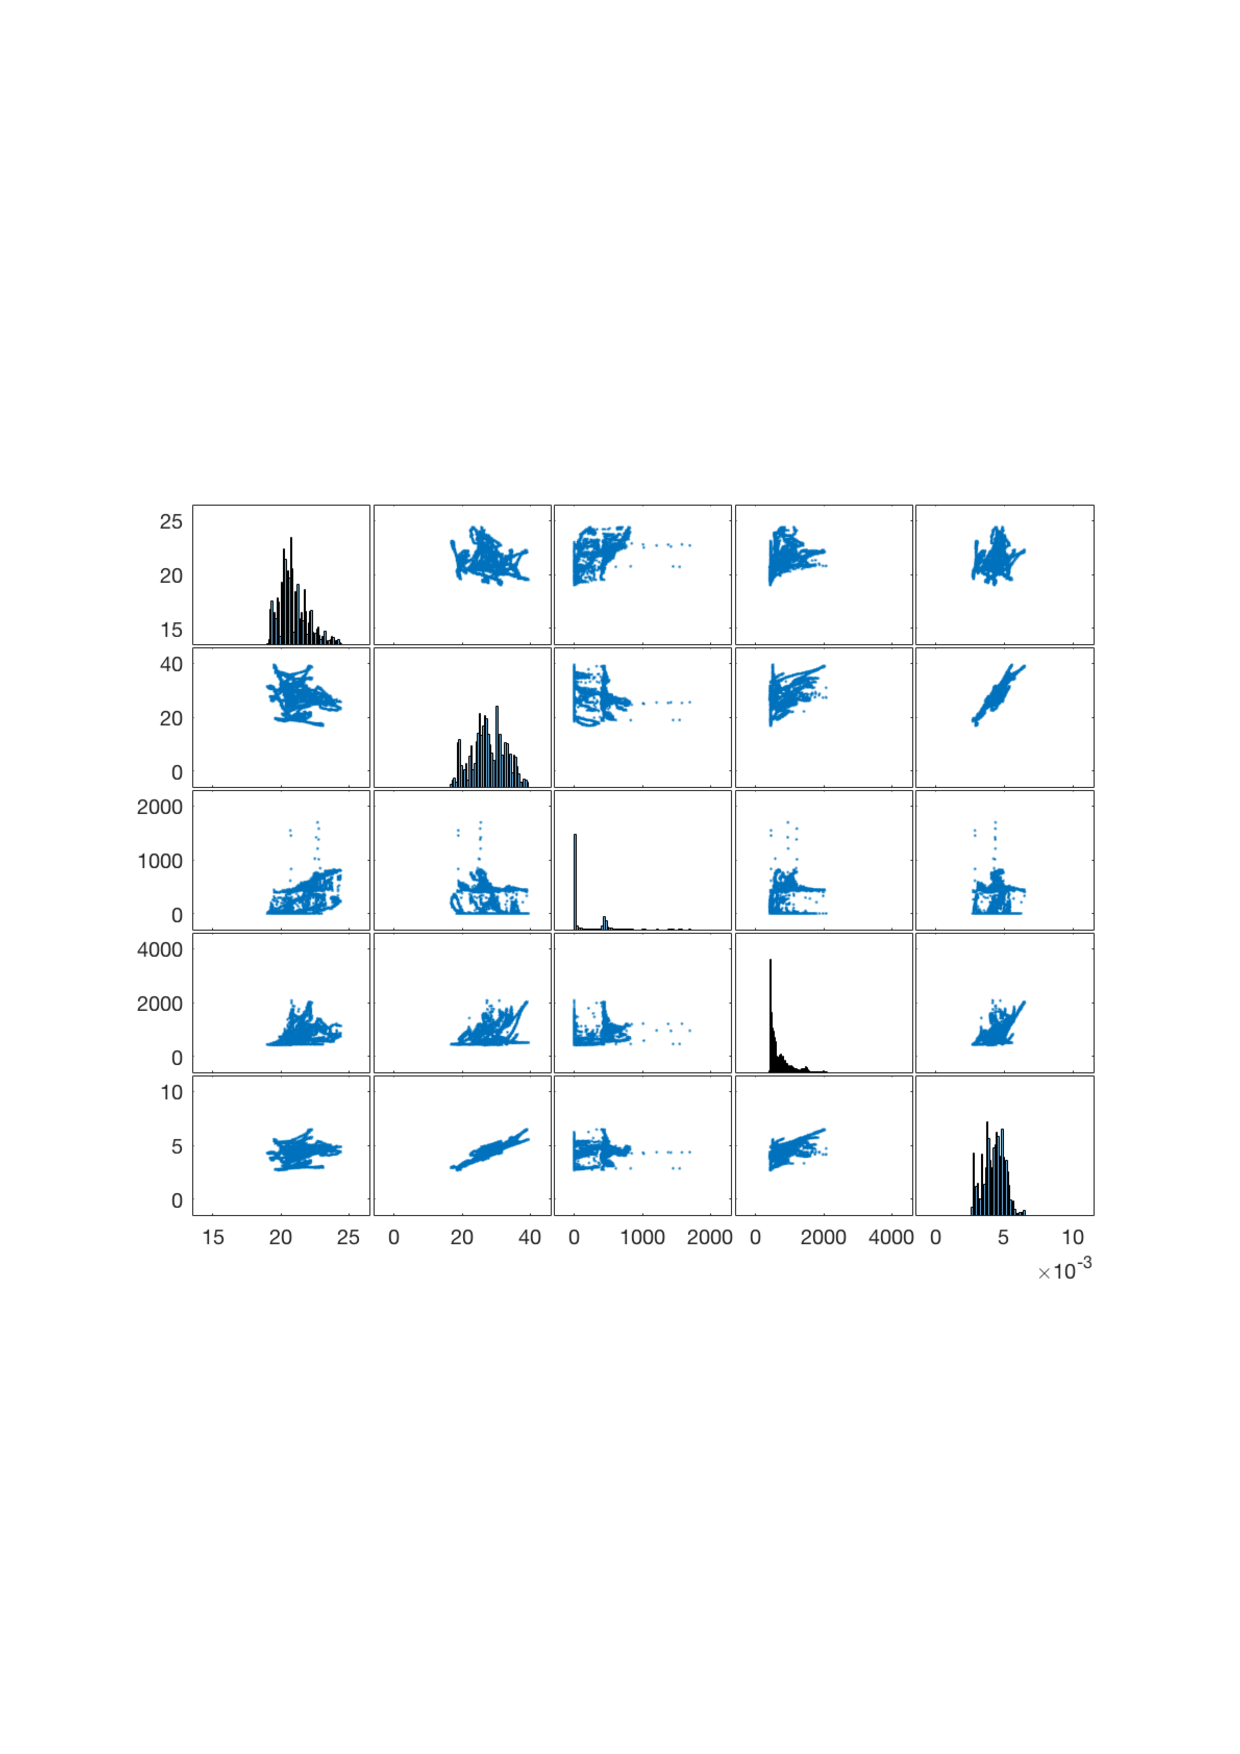
\includegraphics[width=8cm]{plotmatrix1.pdf}
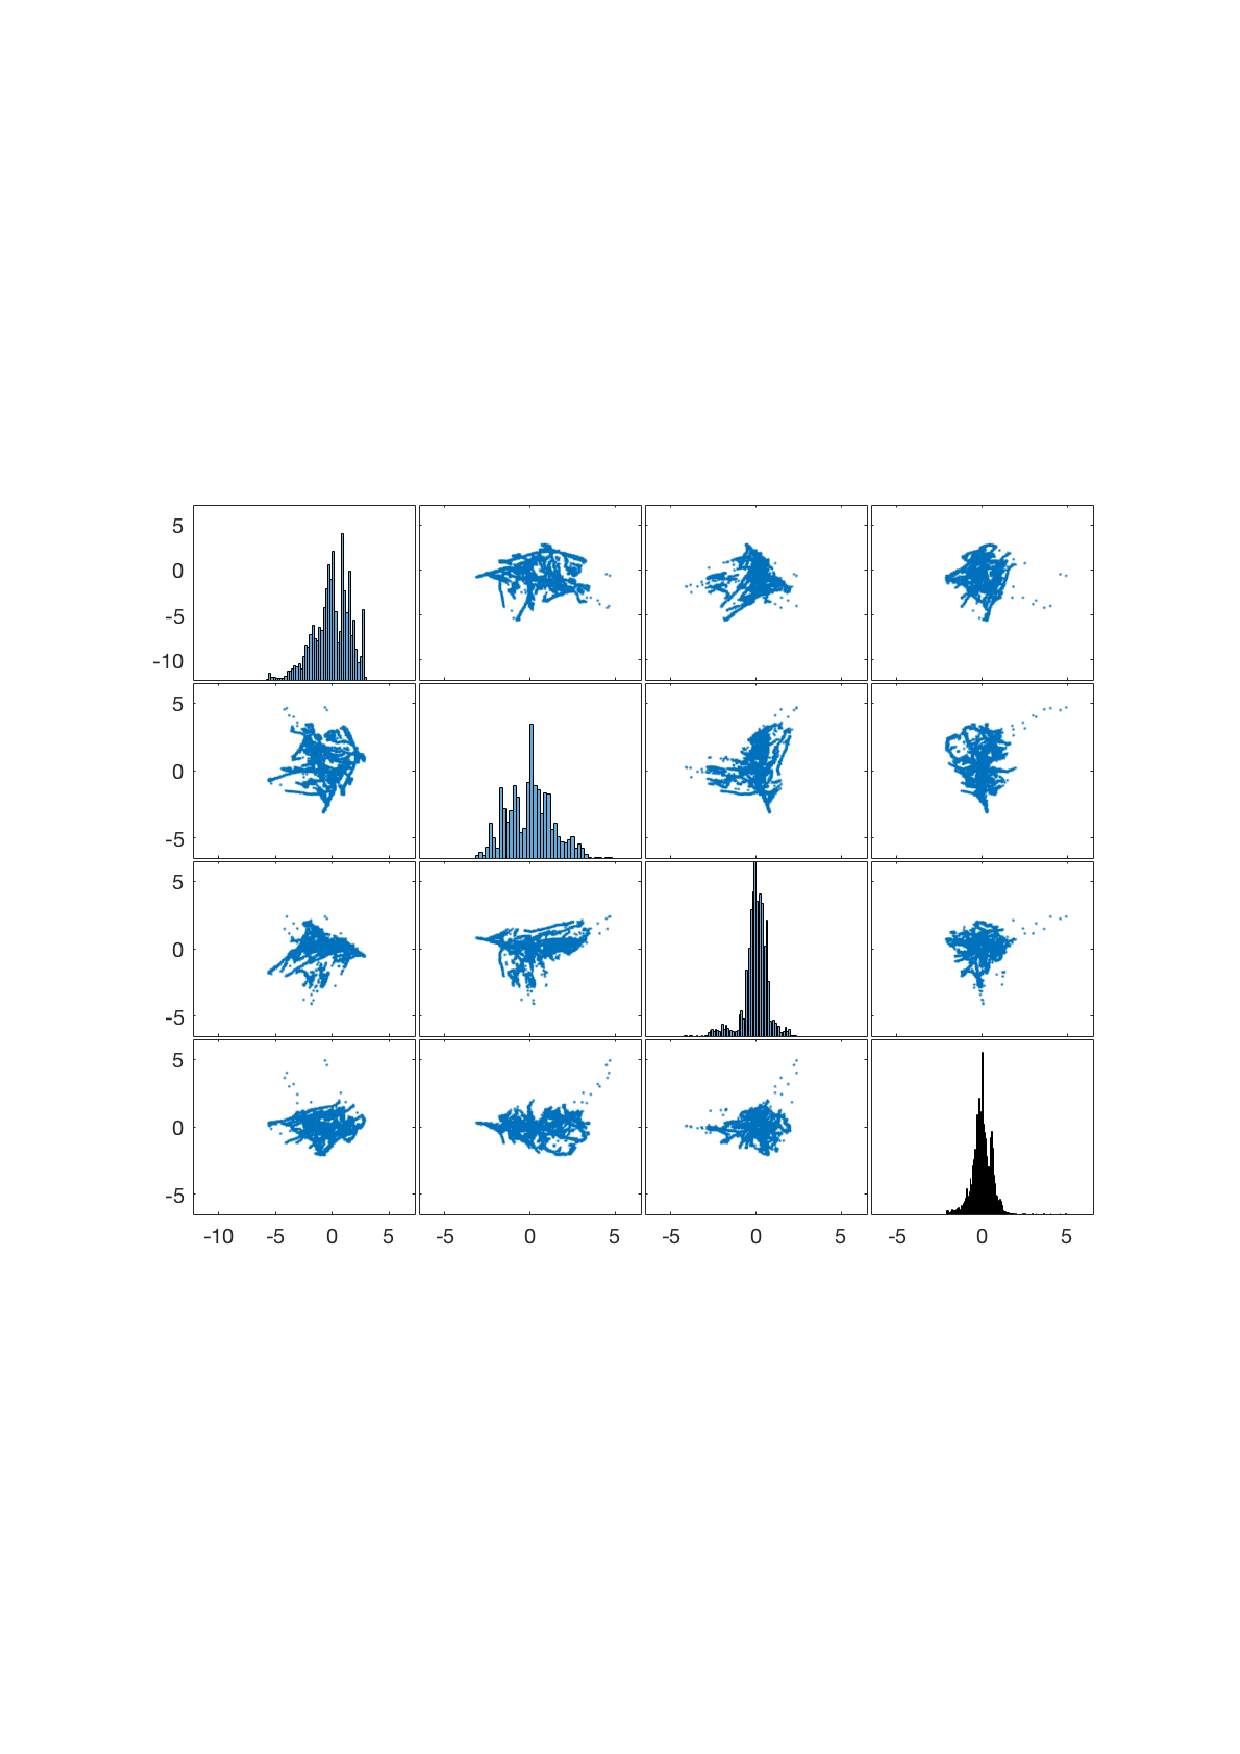
\includegraphics[width=8cm]{plotmatrix2.pdf}
\end{center}
\caption{\label{fig:pca-before-after} Results of $plotmatrix$ of the full dataset before (left) and after (right) PCA.}
\end{figure}

From Figure \ref{fig:pca-before-after} (left), it is clear that some input variables may be skewed, especially \#3 (Light) and \#4 (CO\textsubscript{2}), which may also contain outliers. This makes [0, 1] normalisation with $mapminmax$ potentially unsuitable, as proved by comparison test with unnormalised data, shown in Figure \ref{fig:normalize-testing}.

\begin{figure}[h]
\begin{center}
\fontsize{9}{11}\selectfont
\begin{tabular}{|c|c|c|}
\hline 
Normalisation of Input Dataset & Normalized & Not Normalized \\ \hline
Mean Training MSE & 0.198 & 0.050 \\ \hline \hline 
Mean Validation 1 MSE & 0.138 & 0.064 \\ \hline 
Mean Misclassification 1 (\%) & 16.03 & 2.18 \\ \hline \hline 
Mean Validation 2 MSE & 0.320 & 0.101 \\ \hline 
Mean Misclassification 2 (\%) & 60.53 & 4.58 \\ \hline
\end{tabular}
\end{center}
\caption{\label{fig:normalize-testing} Results from testing the [0, 1] normalisation of training and testing inputs on a [20 1] SOM. (All MSE variances $<0.01$, unnormalised Misclassification 2 variance $=5.74$ , rest $<0.01$.)}
\end{figure}

An alternative to normalisation is to first transform input data so that each variable has a mean of 0 and standard deviation of 1, and then eliminate one or more highly correlated variables, by applying $mapstd$ then $processpca$ with a maximum fraction of 0.02. This resulted in the elimination of one input -- which makes sense, as variable \#5 Humidity Ratio was calculated from temperature and relative humidity, resulting in a possible correlation. The result of PCA is visualised in Figure \ref{fig:pca-before-after} (right). It is evident that the processed input variables are far less correlated, and could potentially improve the training of SOM.

However, it came to a surprise that this is not the case, after a comparison testing of 10 runs with toolbox defaults on a a [20 1] SOM, as shown in Figure \ref{fig:pca-testing}.

\begin{figure}[h]
\begin{center}
\fontsize{9}{11}\selectfont
\begin{tabular}{|c|c|c|}
\hline 
PCA Processing of Input Dataset & After PCA & Before PCA \\ \hline
Mean Training MSE & 0.467 & 0.050 \\ \hline \hline 
Mean Validation 1 MSE & 0.552 & 0.063 \\ \hline 
Mean Misclassification 1 (\%) & 84.65 & 2.17 \\ \hline \hline 
Mean Validation 2 MSE & 0.303 & 0.100 \\ \hline 
Mean Misclassification 2 (\%) & 38.70 & 4.55 \\ \hline
\end{tabular}
\end{center}
\caption{\label{fig:pca-testing} Results from testing the PCA processing of training and testing inputs on a [20 1] SOM. (All MSE variances $<0.01$, pre-PCA Misclassification 2 variance $=5.50$ , rest $<2.20$.)}
\end{figure}

In order to confirm that the high misclassification rates do not originate from a problem in the assumption of SOM clustering on two ends, and that using a two-dimensional SOM instead will not alleviate the issue, SOM sample hit plots from the training of the [20 1] and another [20 5] SOM are shown in Figure \ref{fig:pca-fail}. It can be observed that in both cases, more than two clusters of the data can be seen for each class, rendering a meaningful binary classification impossible.

\begin{figure}[h]
\begin{center}
``Correct'', binary classification, before PCA:\\
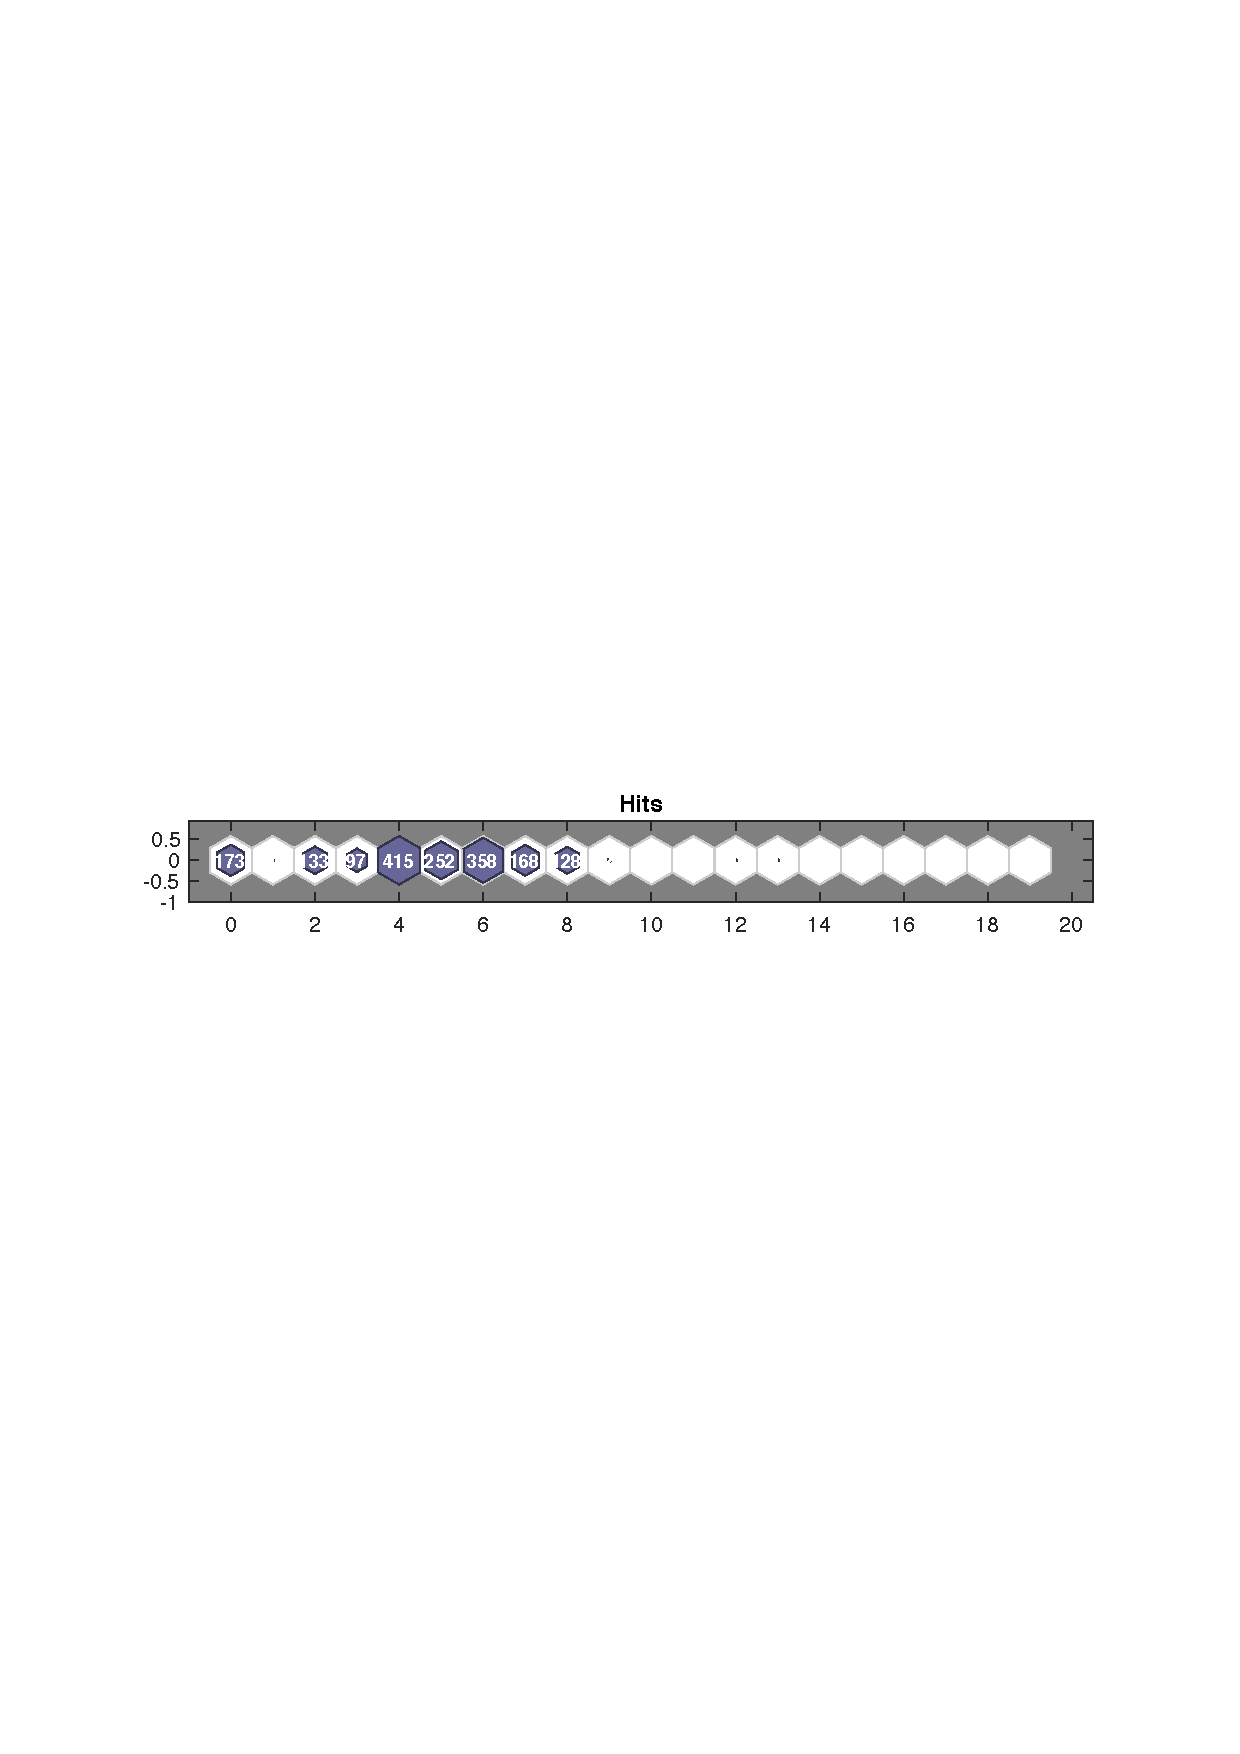
\includegraphics[width=8cm]{nopca-ones.pdf} 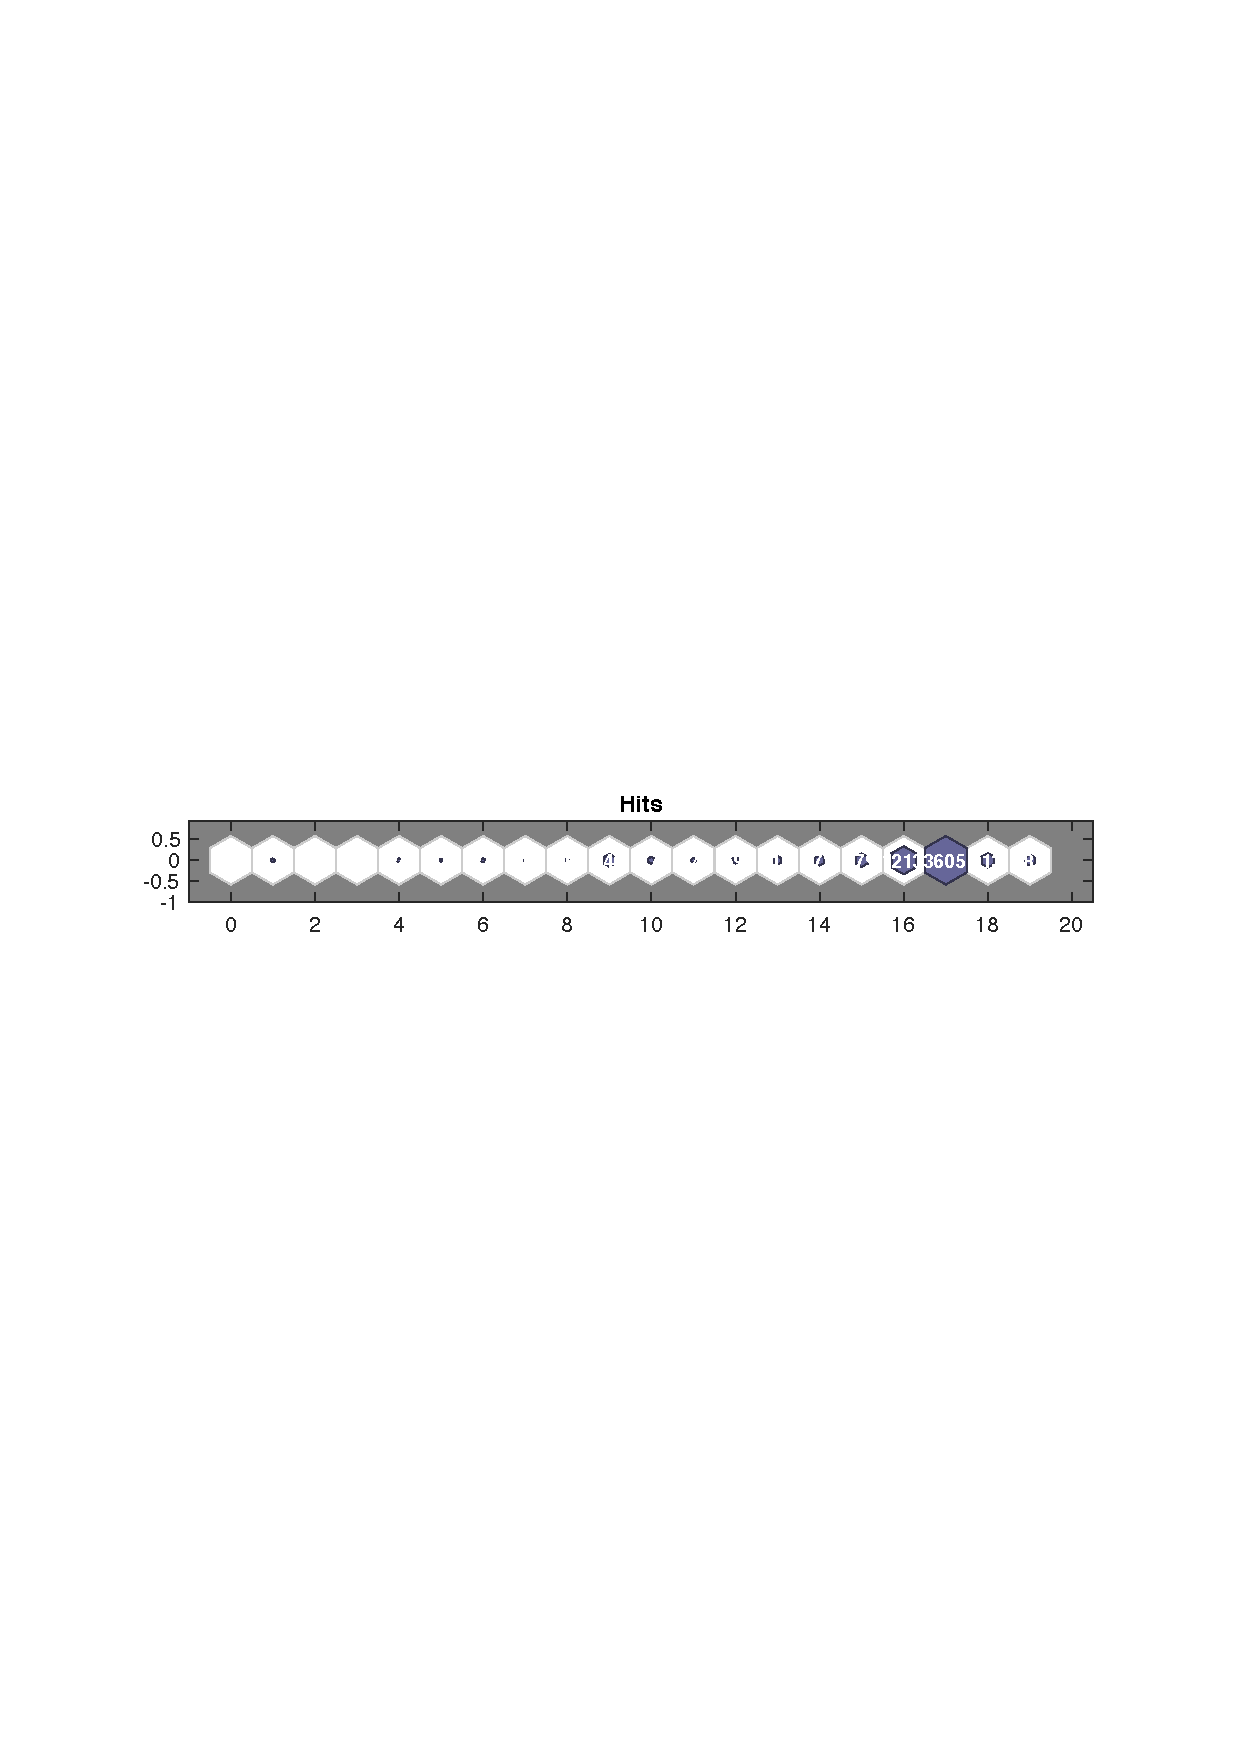
\includegraphics[width=8cm]{nopca-zeros.pdf}\\
``Incorrect'' multi-clustering, after PCA:\\
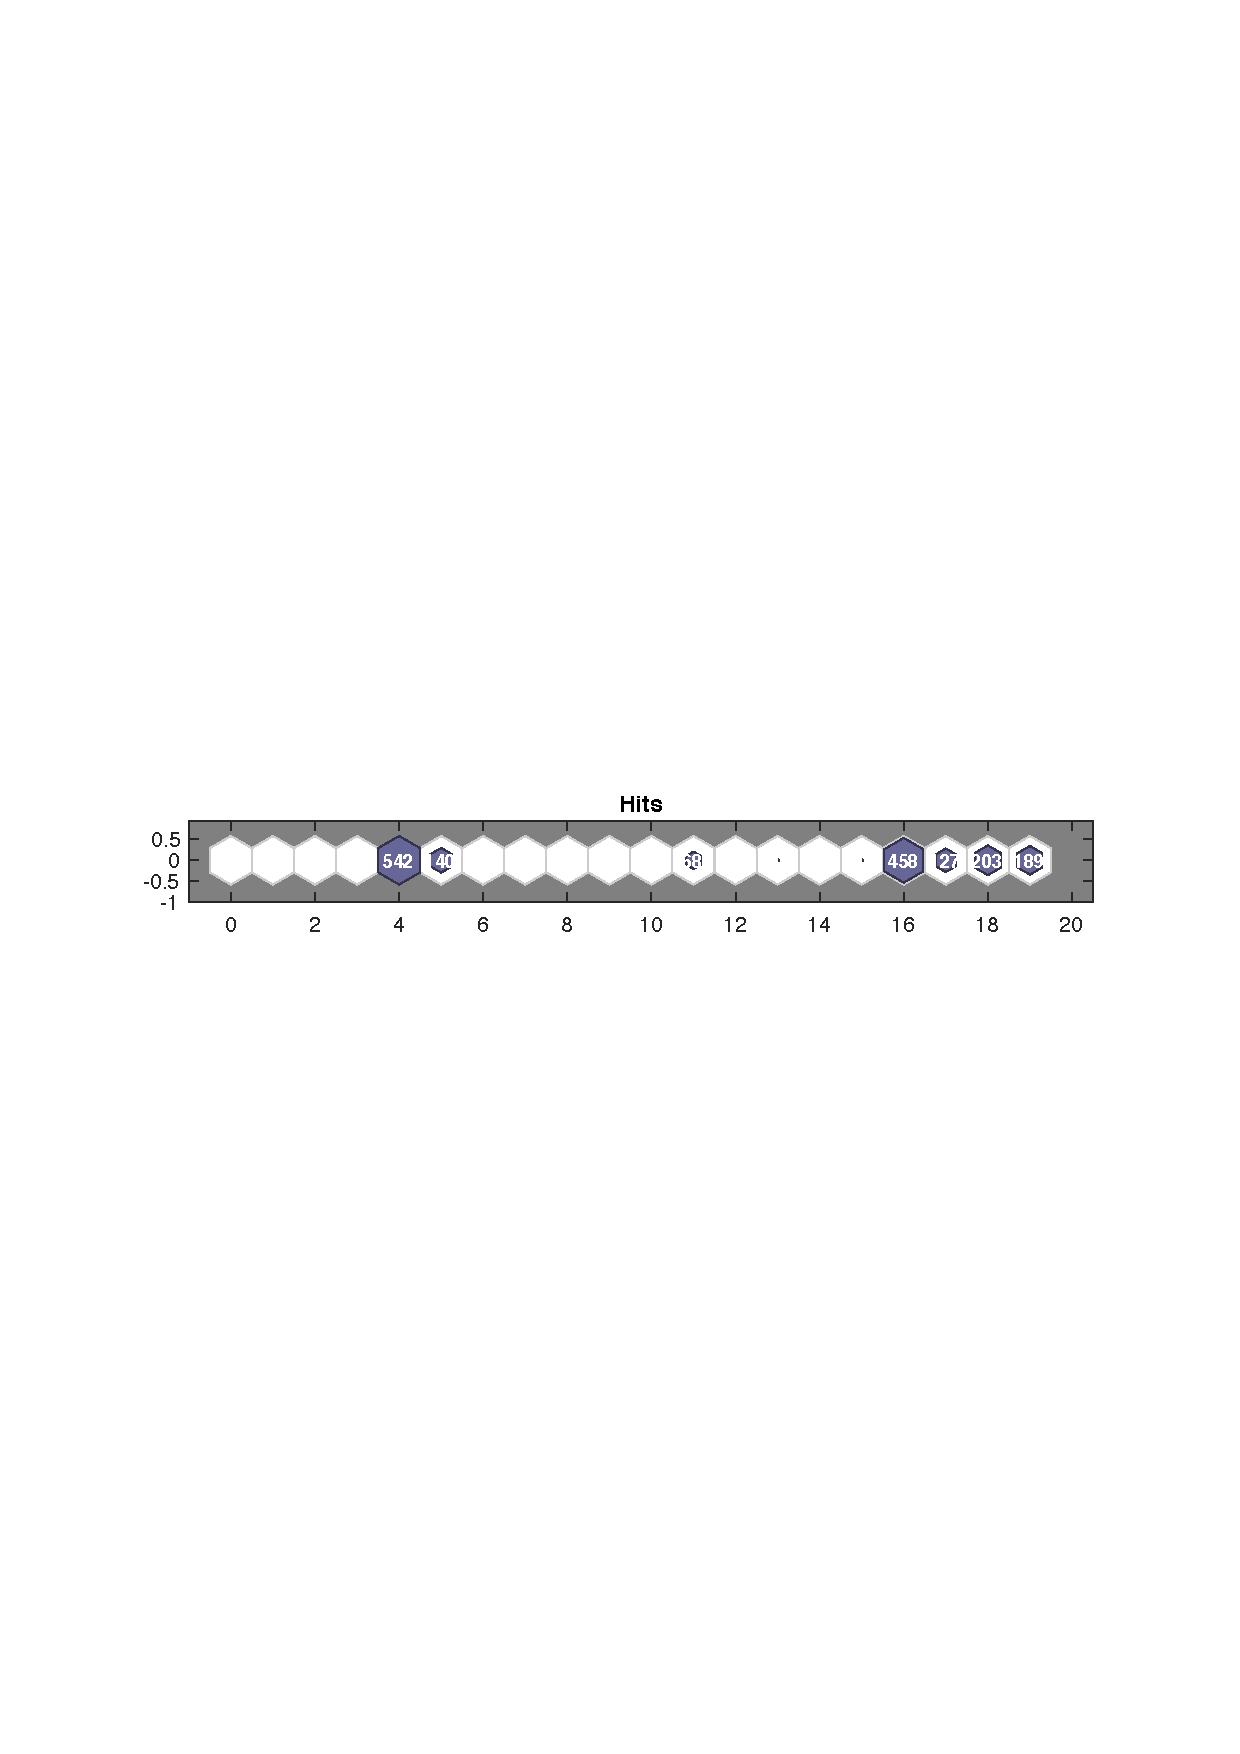
\includegraphics[width=8cm]{pca-fail1-ones.pdf} 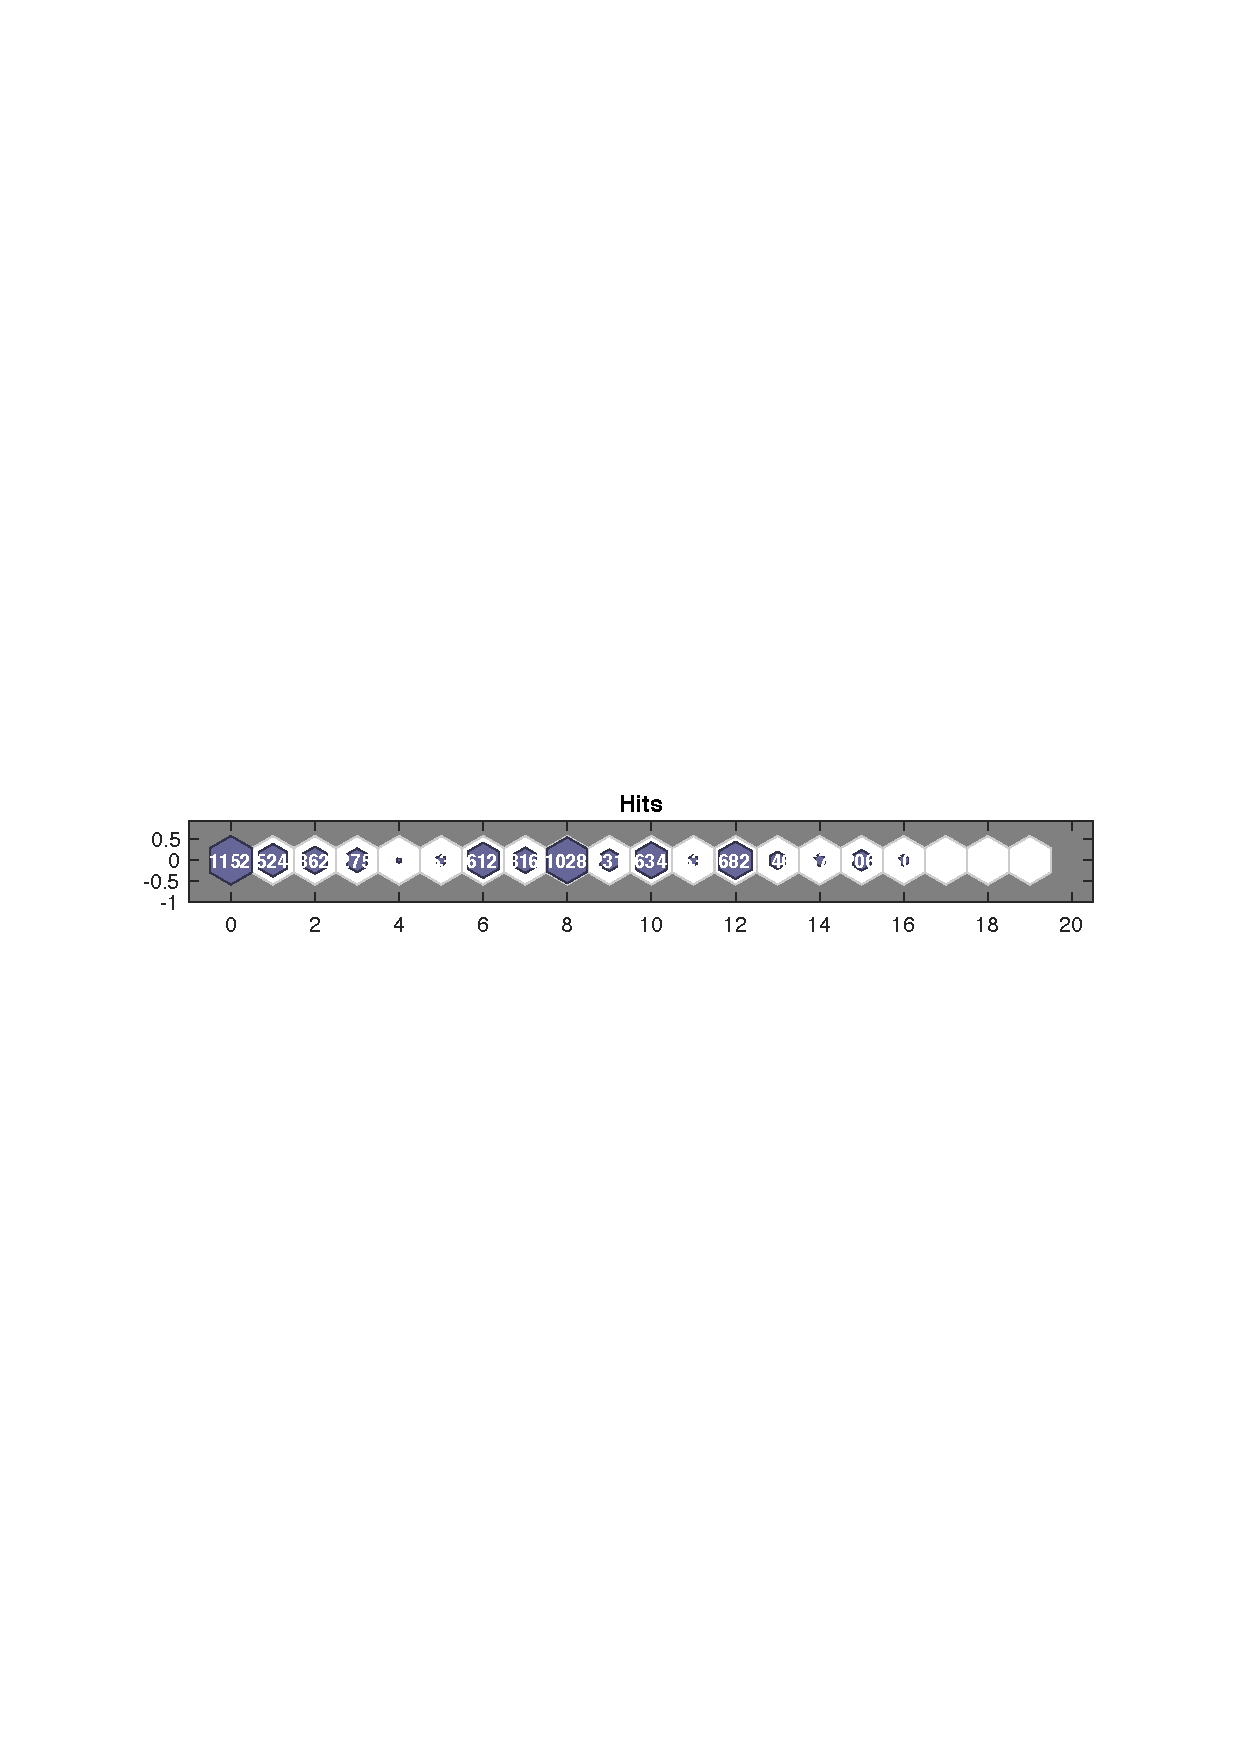
\includegraphics[width=8cm]{pca-fail1-zeros.pdf}
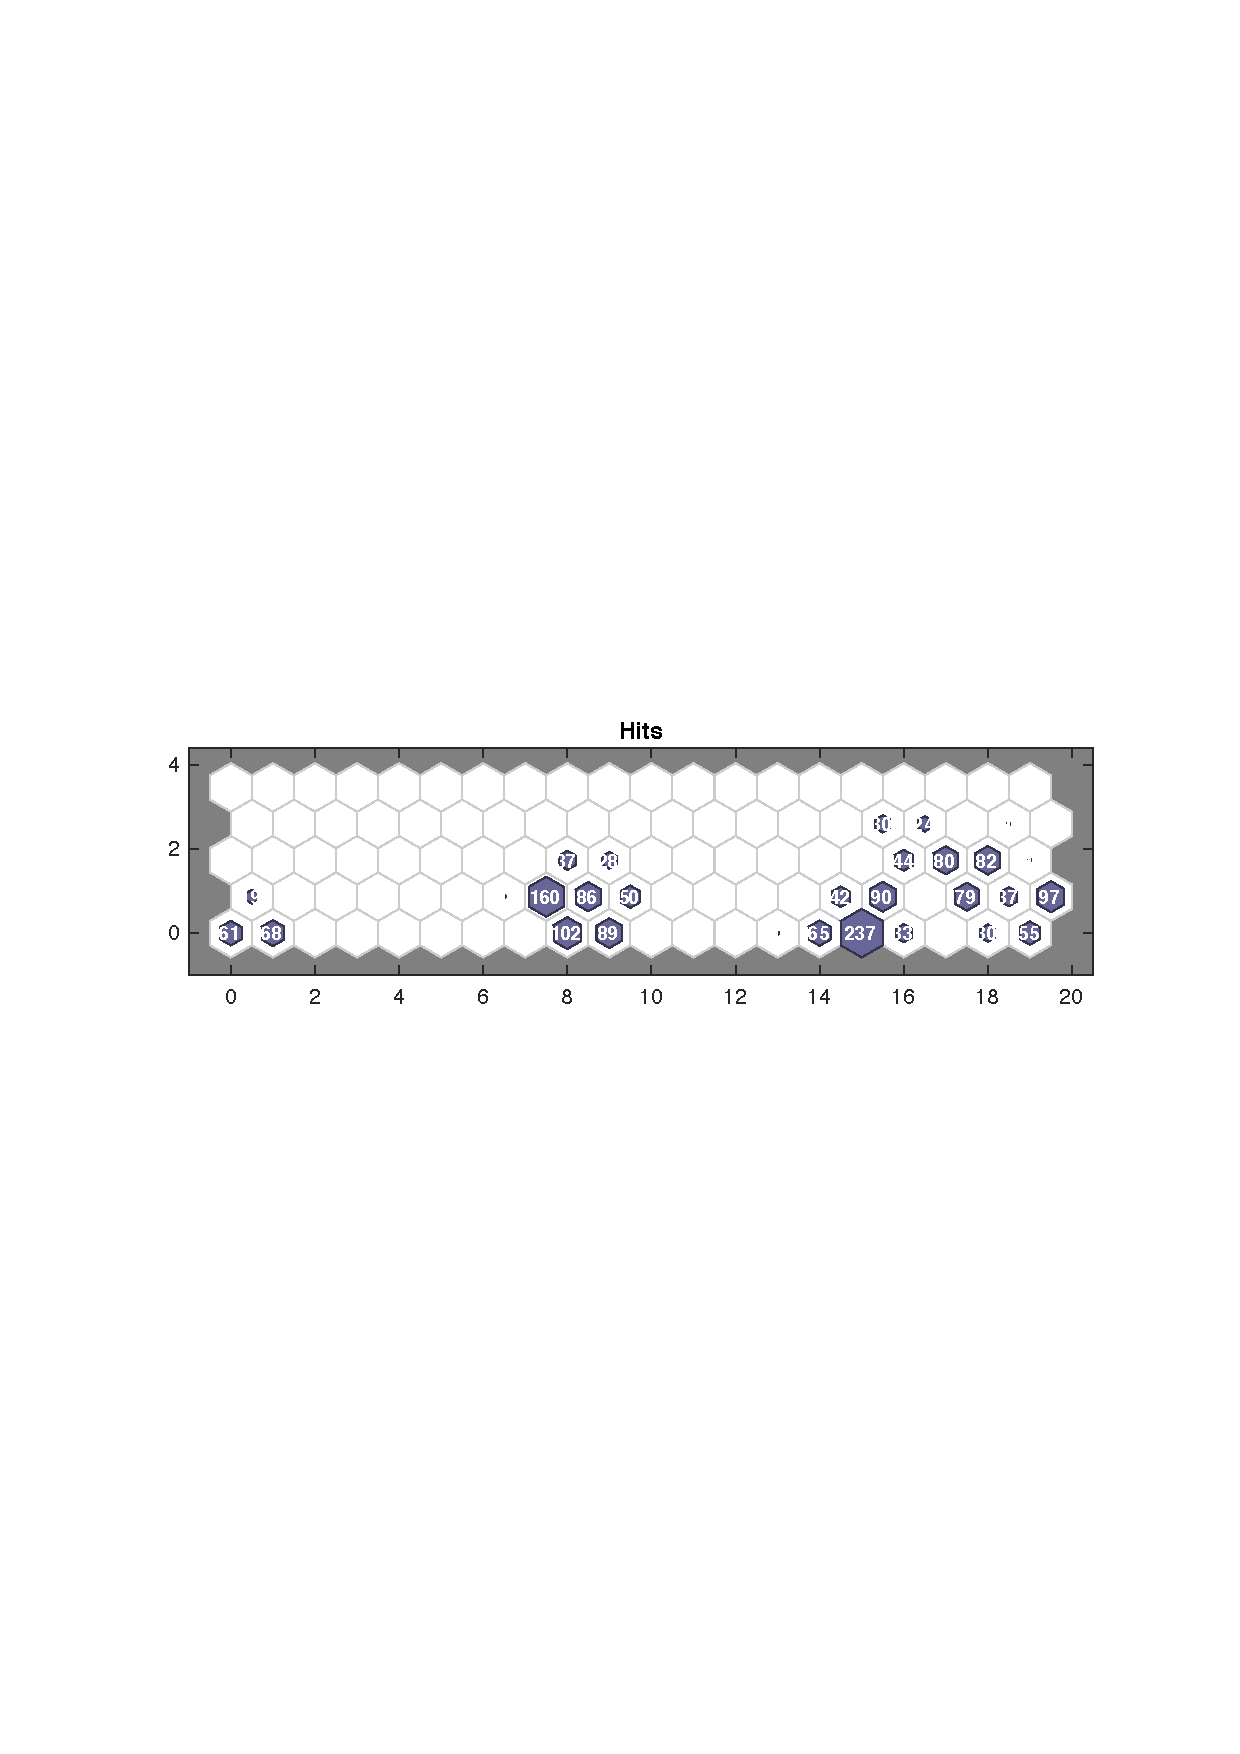
\includegraphics[width=8cm]{pca-fail2-ones.pdf} 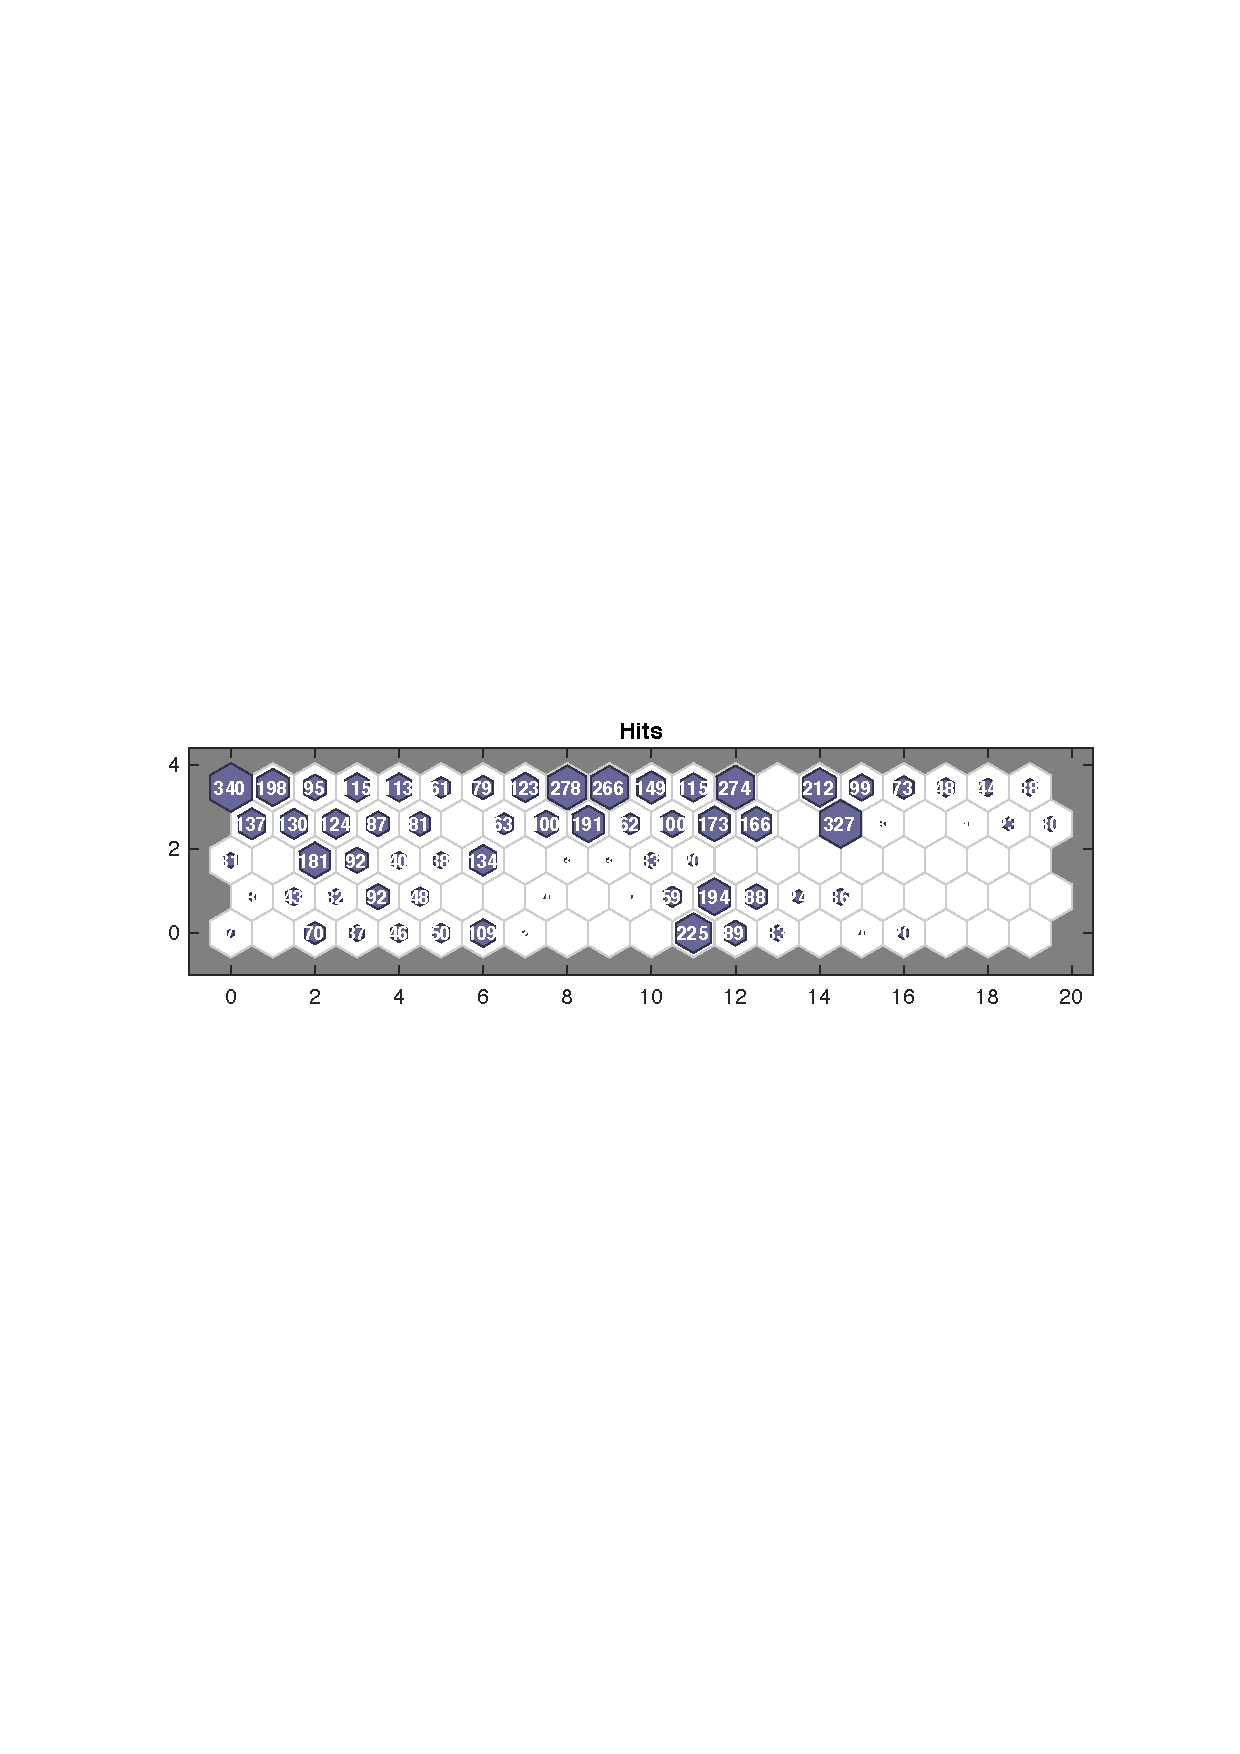
\includegraphics[width=8cm]{pca-fail2-zeros.pdf}
\end{center}
\caption{\label{fig:pca-fail} $plotsomhits$ plots from the training of a [20 1] and a [20 5] SOM on the input data. At the top is the control group (before PCA processing), and at the bottom are SOM plots after PCA (with new SOMs). To the left are occupied cases, and to the right are unoccupied cases.}
\end{figure}

A possible explanation to this interesting observation is that SOM can be considered as a non-linear generalisation of PCA itself \cite[p. 1]{akinduko2012initialization}. Principle component could be used as a method for initialisation of the SOM weight positions, but it was evaluated to perform less well than random initialisation \cite[p. 1]{akinduko2012initialization}. Therefore, applying PCA on the inputs of SOM may not achieve the same effects as on the inputs of a MLP. 

Considering the fact that the five variables shown in Figure \ref{fig:final-variables} without additional pre-processing already performs very well (low-single-digit misclassification percentages), confirmed by the control groups of the comparisons performed in this section, it was decided that \textbf{the five input variables will be used as is for the SOM without further processing}.

\subsection{Description of the SOM architecture}

The self-organising map (SOM) represents a unique feedforward architecture \cite[p. 429]{haykin2008}. The architecture consists of a mesh of connected neurons, each selectively tuned for specific features of the input data during the training process \cite[Sec. 9.1]{haykin2008}. The mesh of neurons are topologically ordered \cite[p. 11]{som-lecture}, which implies that a specific point on the mesh maps to a specific set of characteristics seen in a certain set of input data. This feature allows SOM to be used to solve simple classification problems such as this one, in addition to its very useful purposes in projecting high-dimensional data nonlinearly to achieve purposes such as visualisation. Two models of this mapping process exist: the Willshaw-von der Malsburg's model and the Kohonen model \cite[Sec. 9.2]{haykin2008}, and the MATLAB toolbox uses the Kohonen model \cite{som-matlab} -- to be described in more detail in Section \ref{subsec:training}.

The SOM is implemented through the $selforgmap$/$newsom$ and associated methods in the MATLAB Neural Network Toolbox \cite{kohonen2014matlab}. For all of the preliminary testings in the previous sections, the default parameters for the network were used: 100 epochs in each phase of the training (phases to be covered in \ref{subsec:training}), initial neighbourhood size of 3 (to be gradually reduced), neurons arranged in a hexagonal topology with linked distance as the distance function. Later in Section \ref{subsec:training}, changes to some of these parameters will be explored.

The architecture of the SOM is relatively simple to implement: an input layer of a set number of neurons connecting to a single layer of map neurons (nodes) topographically arranged in a mesh, the dimensions of which are defined by the network configuration. Each map neuron has a set of weights for its connections with input layer neurons, which affect the length of each connection, resulting in the surface of the mesh to ``bend'' as the weights change. At initialisation, various methods can be used to initialise these weights. The toolbox default creates linearly separated sets of weight, shown in Figure \ref{fig:som-init} (right), and places the same number of neurons on the input layer as there are input variables.

Lateral connections are also created between neighbouring neurons based on the topology. Their positions are useful to the distance function, in this case linked distance (which means distances are immutable in this case, as $linkdist$ counts by neuron only). For the one-dimensional mesh used in this report, the lateral connections are much simpler due to the simplified structure (at most two connections per neuron), as shown in Figure \ref{fig:som-init} (left). A visual illustration of another SOM with dimensions [5 2] is shown in Figure \ref{fig:som-visual}.

\begin{figure}[h]
\begin{center}
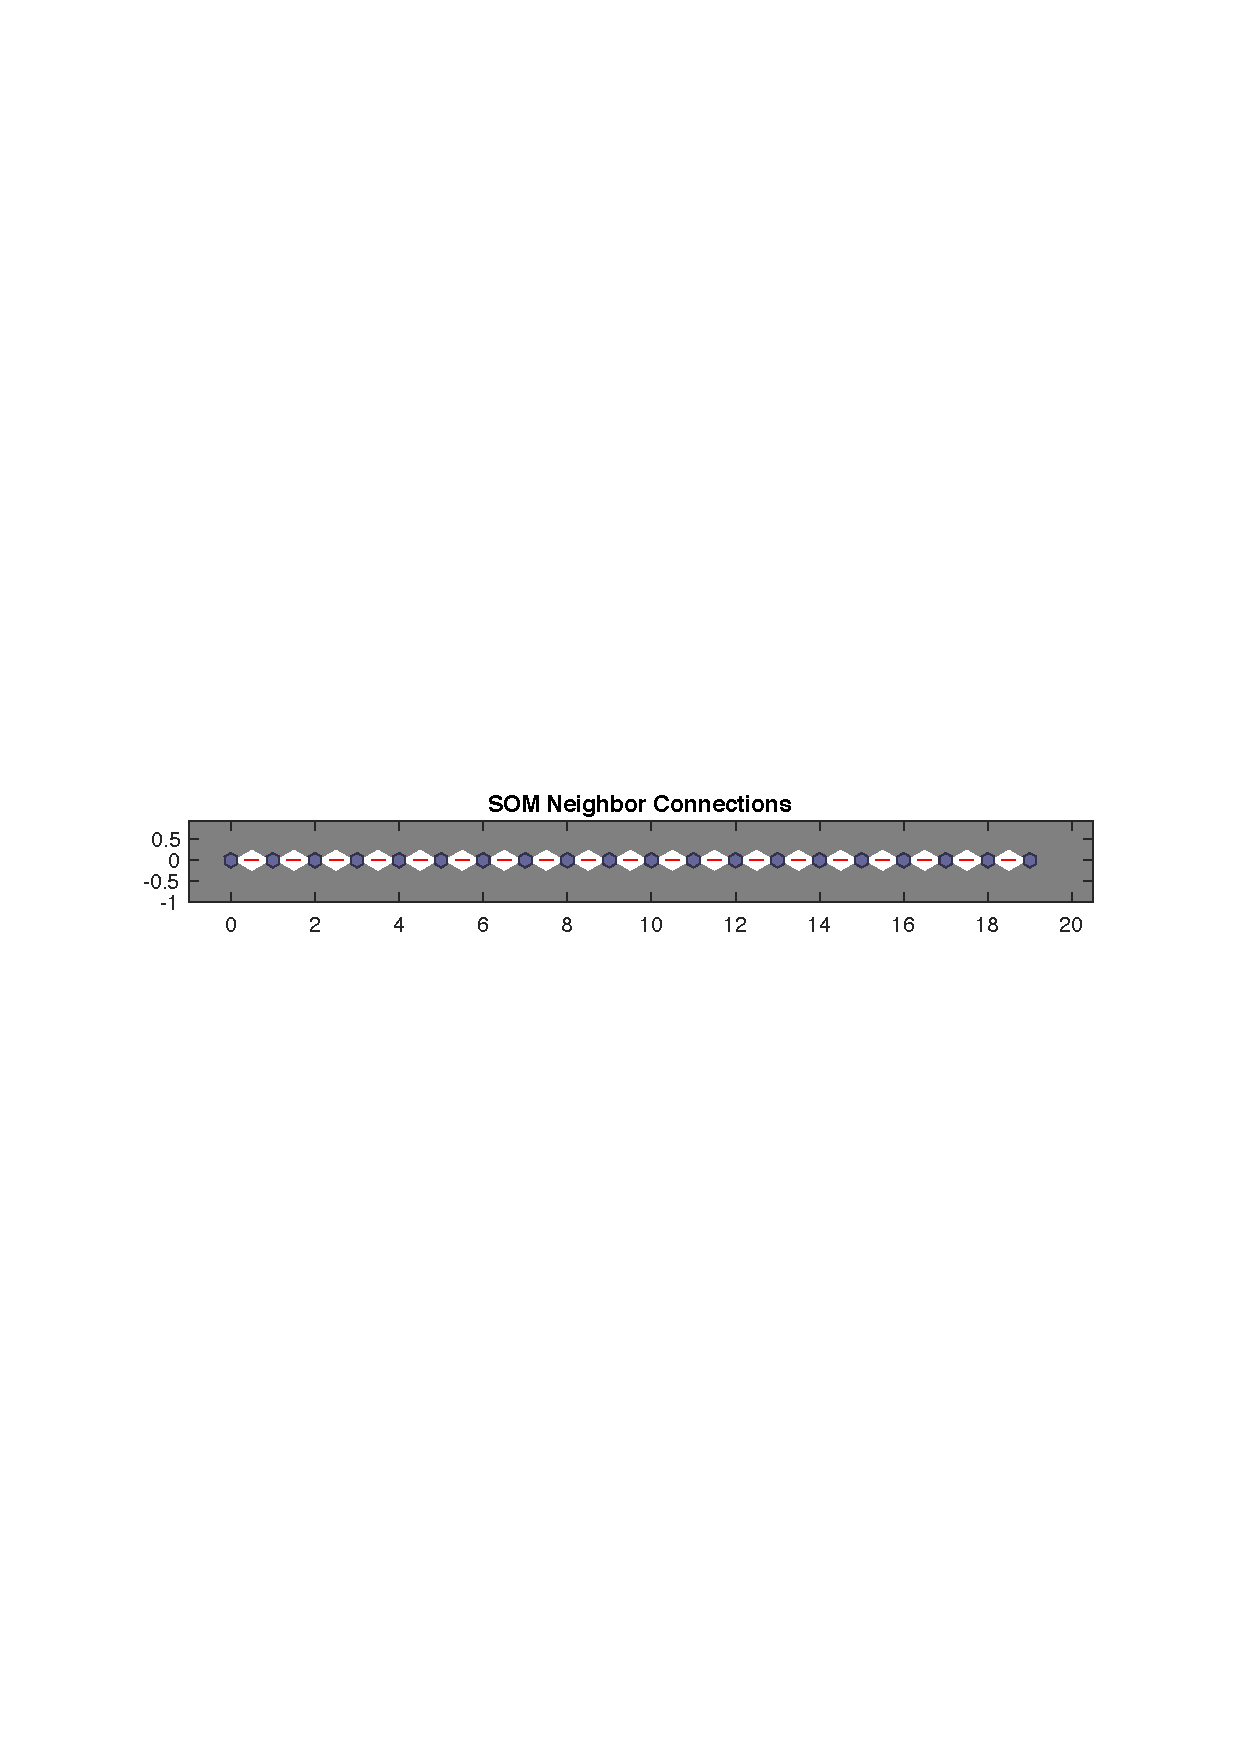
\includegraphics[width=12.5cm]{somnc.pdf} 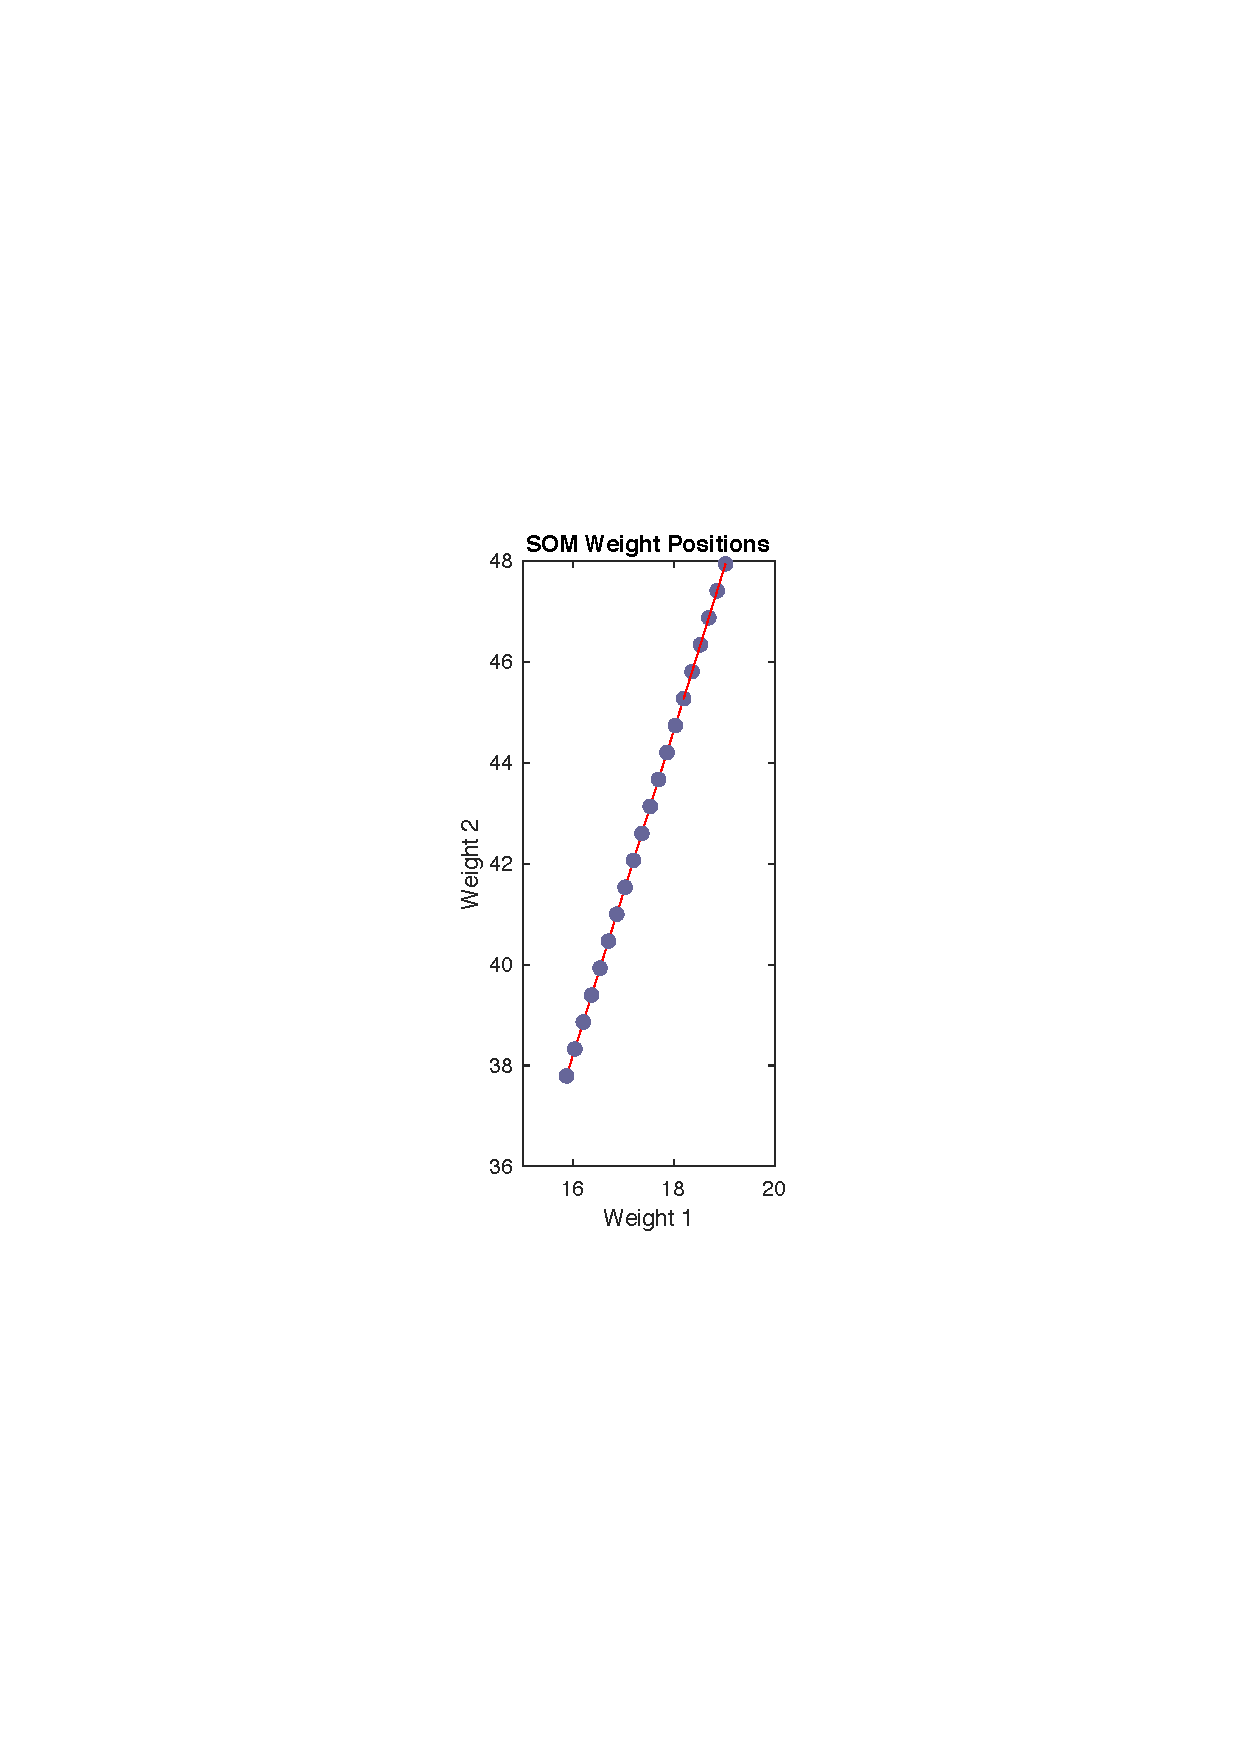
\includegraphics[width=2.07cm]{sompos.pdf} 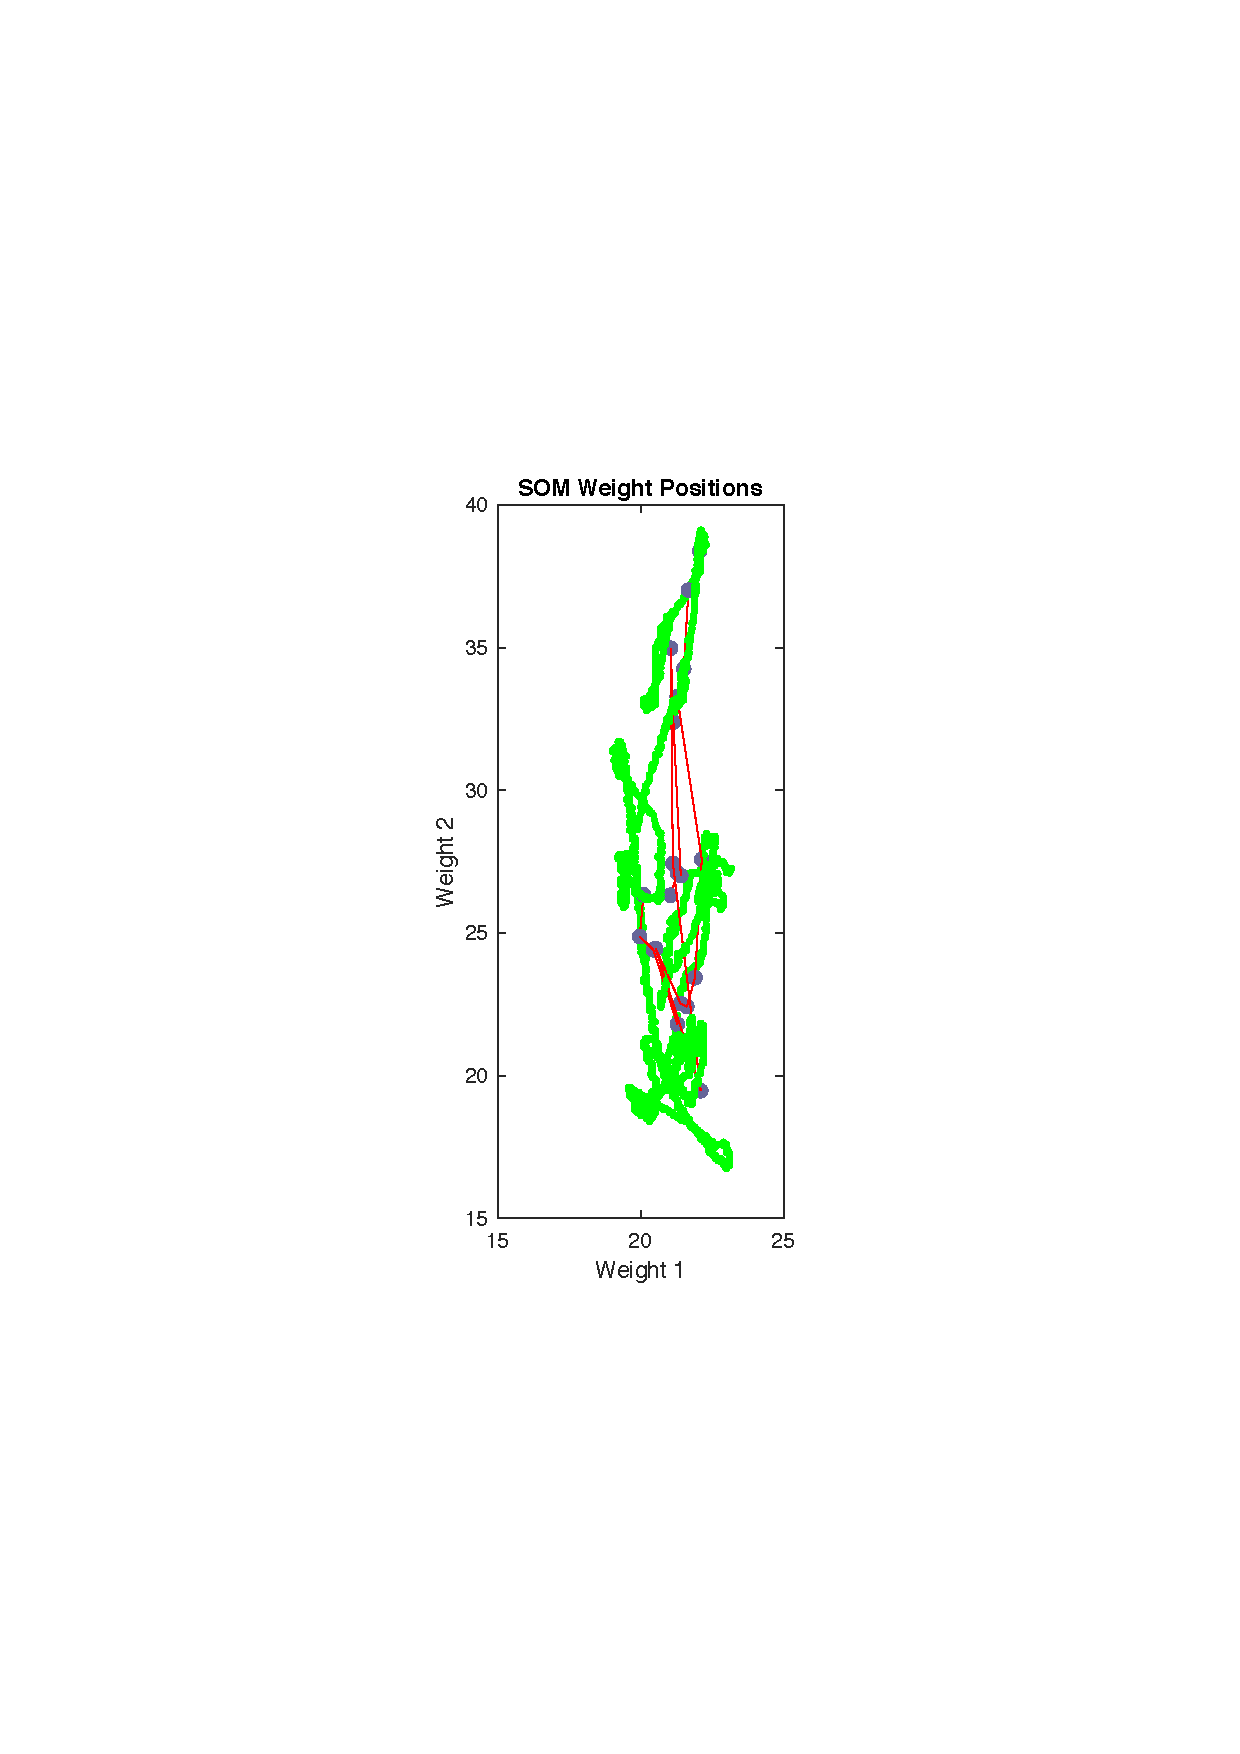
\includegraphics[width=2cm]{sompos-aftertraining.pdf}
\end{center}
\caption{\label{fig:som-init} The initial neighbour connections (left) and weight positions (mid, first two weights of five) of the SOM created by the toolbox, as well as the weight positions of the same inputs after training (right).}
\end{figure}

\begin{figure}[h]
\begin{center}
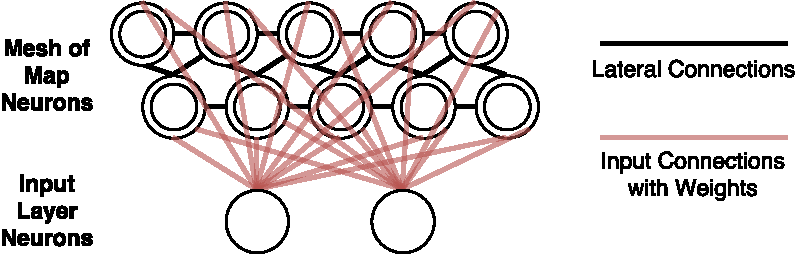
\includegraphics[width=12cm]{som-visual.pdf} 
\end{center}
\caption{\label{fig:som-visual} Visual illustration of a SOM with dimensions [5 2] and two input neurons (possibly connecting two input variables). The mesh is arranged in $hextop$ grid.}
\end{figure}

\subsection{Training of the SOM architecture} \label{subsec:training}
 
Unlike MLP, a Kohonen SOM has a defined way of training, implemented in the toolbox as $trainbu$. The training is divided into two, usually equal-length phases: the ordering phase and the convergence phase \cite[p. 23]{som-lecture}. The purpose of the training process is to expose all neurons to a sufficient number of different input patterns with different corresponding active spots on the map \cite[p. 429]{haykin2008}, adjusting the input weights and therefore allowing the network to produce distinct responses on different classes of input patterns. Haykin \cite[p. 435]{haykin2008} recommends 1000 steps for each phase of the training. The MATLAB toolbox default is 100 for each phase \cite{som-matlab}, which produced a general classification accuracy of $>95$\% in cursory and data processing testing as shown in the previous sections.

The two training phases are procedurally identical, but different in the values of learning rate ($\eta$) and neighbourhood size ($\sigma$), both of which smaller in the convergency phase than the ordering phase, as the ordering phases is responsible for main topological ordering, while the convergency phase is used for fine tuning between neighbouring neurons \cite[p. 23]{som-lecture}. The initial learning rates are $\eta=0.9$ and $\eta=0.02$, and the initial neighbourhood sizes are the entire mesh's radius and $\sigma=1$ for the ordering and convergence phases respectively \cite{newsom-matlab}. These values are close to the recommended start values\cite[p. 23]{som-lecture}. During each phase, exponential functions gradually reduce these parameters, as described below.

Each step during either phase is a three-stage process: competition, cooperation and adaptation \cite[pp. 429-430]{haykin2008}. The first stage determines the most excited (winning) neuron, which is used to determine a neighbourhood in the second stage, through a neighbourhood function $h$. Neurons in the neighbourhood selected then have their weights adjusted to be closer to the most excited neuron in the last stage. This process repeats until a defined number of steps are completed for each phase.

In the competition phase, with an input space of $m$ variables and the particular input $x$, the selection of the most excited neuron $i(x)$ on a mesh of neurons (each neuron $j$ with a weight vector $w_j$) is with the following algorithm \cite[p. 430]{haykin2008}:
\begin{equation}
i(x) = arg \min_{j}\|x  - w_{j}\| \ \text{, where}\ x = [x_1, x_2, ..., x_m]^T \ \text{and} \ w_j = [w_{j1}, w_{j2}, ..., w_{jm}]^T
\end{equation}

In the cooperation phase, owing to the observation that neurons closer to the winning neuron assimilate more towards the winning neuron than the neurons further away, the neighbourhood function $h$ determines the scale of activation, based on the set neighbourhood size $\sigma$, and the distance from the winning neuron $d_{ji}$ as determined by a distance function, such as linked distance ($linkdist$) \cite[p. 431]{haykin2008}:
\begin{equation}
h_{ji} = exp(-\frac{d^2_{ij}}{2\sigma^2}) \ \text{for lateral distance between the winning neuron $i$ and neighbouring neuron $j$}
\end{equation}

And finally, in the adaptation phase, neurons in the neighbourhood of the winning neuron will assimilate towards the winning neuron. The new weight $w_j(n+1)$ of neuron $j$ is updated at the $n+1$ step as followed \cite[p. 21]{som-lecture}:
\begin{equation}
w_j(n+1) = w_j(n) + \eta h_{ji}(n)(x-w_j(n))
\end{equation}

To achieve a gradual process of weight adjustment, the learning rate $\eta$ and the neighbourhood size $\sigma$ are usually exponentially reduced over time \cite[pp. 21-22]{som-lecture}:
\begin{equation}
\eta (n) = \eta_0 exp(-\frac{n}{\iota}) \;\;\;\;\;\;\;  \sigma (n) = \sigma_0 exp(-\frac{n}{\iota'})
\end{equation}

While there is no choice of training algorithms, it is possible to alter the number of steps in each phrase of training, as well as the initial neighbourhood sizes $\sigma$ to observe their effects on the performance of the trained SOM. Unfortunately the newer implementations of $newsom$ in the toolbox no longer allows the adjustment of initial learning rates at each phase, fixating them at $\eta=0.9$ and $\eta=0.02$ respectively\cite{newsom-matlab}. Based on the recommendations from the module \cite{som-lecture} and Haykin \cite{haykin2008}, several different combinations of training steps, learning rates and neighbourhood sizes are chosen, each tested ten times on a fresh [20 1] SOM. 

First, to test the influence of number of steps in each phase, a few training configurations are tested with the default learning rates and neighbourhood sizes, as shown in Figure \ref{fig:steps-testing} and plotted in Figure \ref{fig:testing-plots} (left). Based on the mean validation performance on unseen data, 500 steps is selected as the number of steps in each phase of training, as it produces the best possible result in the second, larger validation set, and produces the second best result in the first validation set. Compared with the recommended 0.1 initial learning rate at 1000 steps accumulating to an ``amount'' of 100, 500 steps at the default 0.9 initial learning rate accumulates to 450 -- 3.5 times longer.

\begin{figure}[h]
\begin{center}
\fontsize{9}{11}\selectfont
\begin{tabular}{|*{8}{c|}}
\hline 
Number of Steps in Each Training Phase & Data & 100 & 250 & 500 & 750 & 1000 & 2000 \\ \hline
\multirow{2}{*}{Training MSE} & Mean & 0.050 & 0.068 & 0.066 & 0.071 & 0.069 & 0.071 \\ \cline{2-8}
\ & Variance & \multicolumn{6}{c|}{$<$0.01} \\ \hline
\multirow{2}{*}{Validation 1 MSE} & Mean & 0.064 & 0.094 & 0.092 & 0.098 & 0.096 & 0.098  \\ \cline{2-8}
\ & Variance & \multicolumn{6}{c|}{$<$0.01} \\ \hline
\multirow{2}{*}{Misclassification 1 (\%)} & Mean & 2.18 & 3.45 & 3.39 & 3.97 & 3.88 & 3.65 \\ \cline{2-8}
\ & Variance & $<$0.01 & 0.283 & 0.222 & 0.952 & 0.947 & 0.106 \\ \hline
\multirow{2}{*}{Validation 2 MSE} & Mean & 0.101 & 0.127 & 0.118 & 0.134 & 0.128 & 0.131 \\ \cline{2-8}
\ & Variance & \multicolumn{6}{c|}{$<$0.01} \\ \hline
\multirow{2}{*}{Misclassification 2 (\%)} & Mean & 4.54 & 4.96 & 3.88 & 5.88 & 5.28 & 5.12 \\ \cline{2-8}
\ & Variance & 5.38 & 7.02 & 3.36 & 11.7 & 10.4 & 8.74 \\ \hline
\end{tabular}
\end{center}
\caption{\label{fig:steps-testing} Results from varying the number of steps in each phase of training on a [20 1] SOM. The total number of training epochs is twice this number.}
\end{figure}

\begin{figure}[h]
\begin{center}
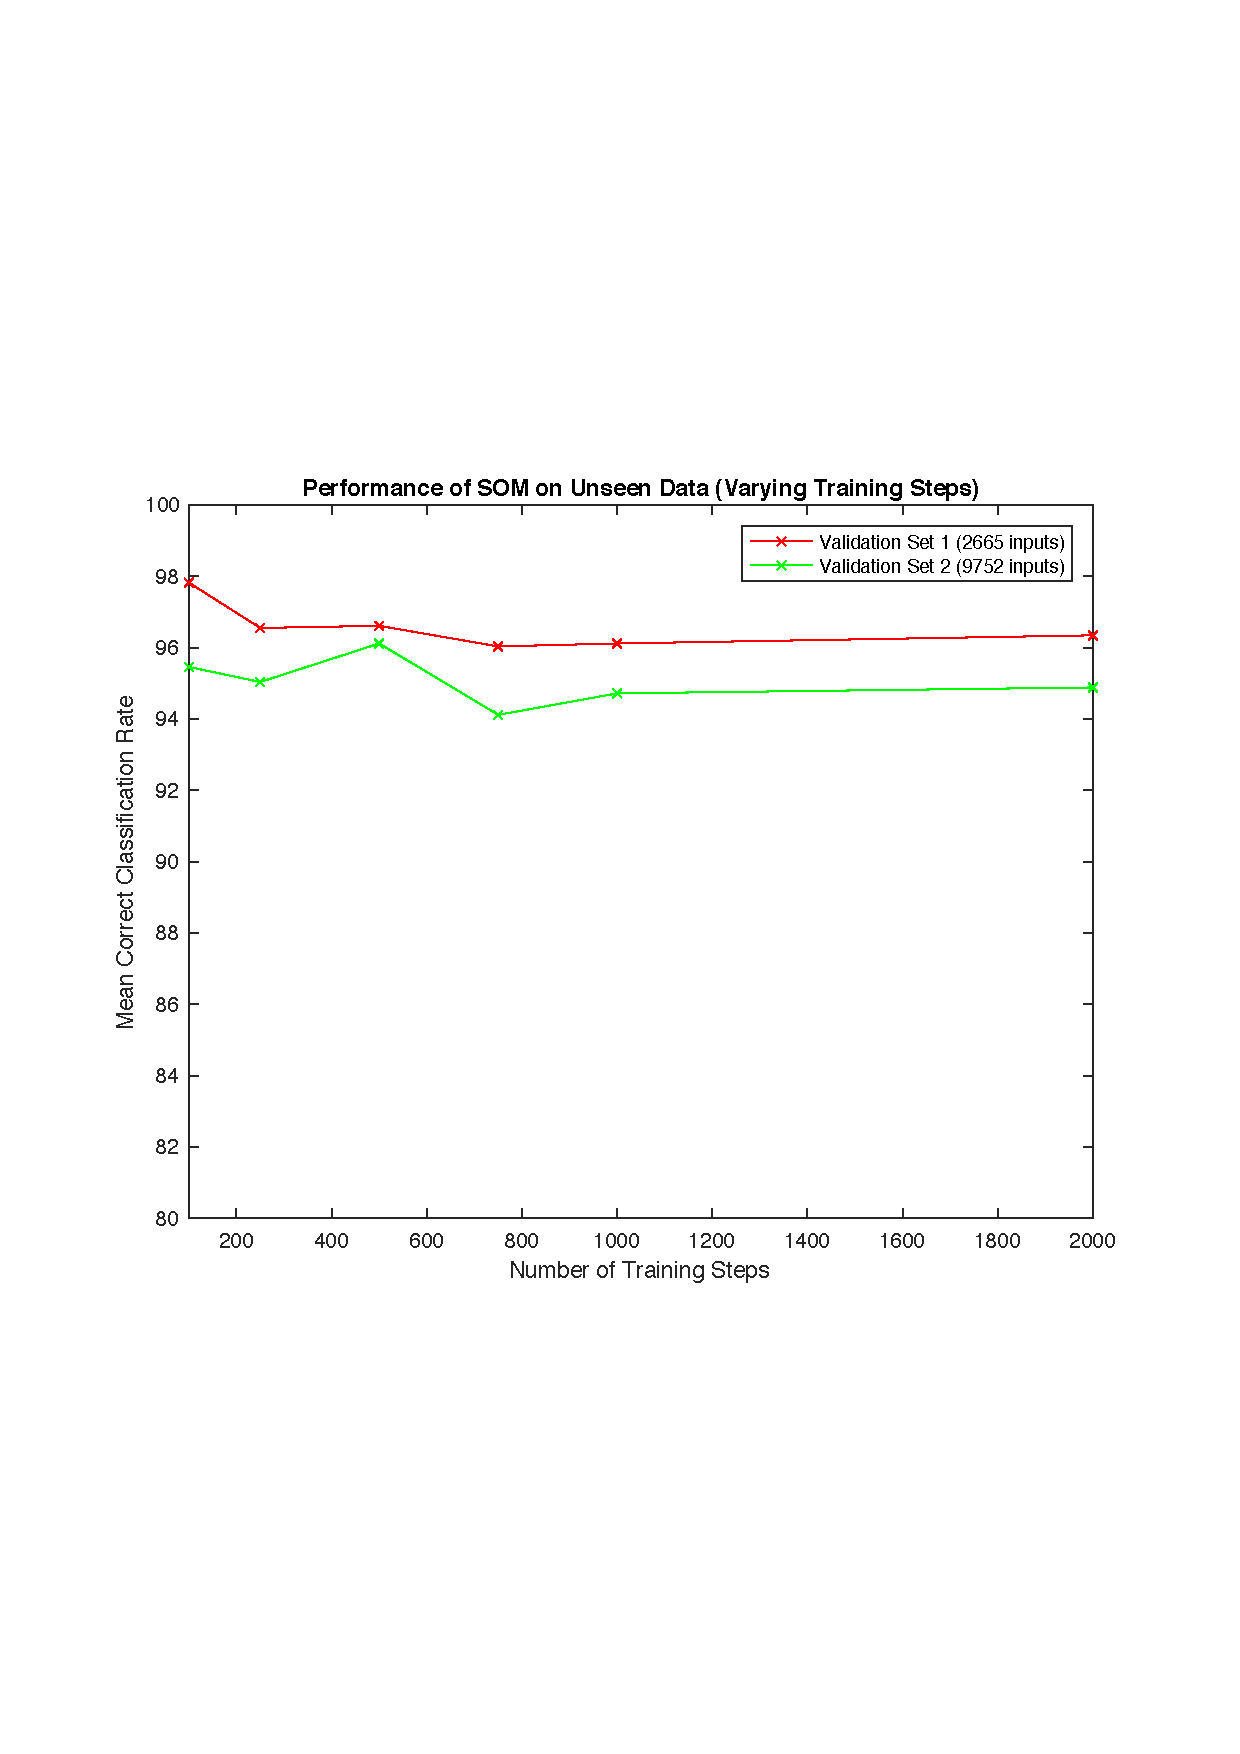
\includegraphics[width=7.5cm]{steps-plot.pdf} 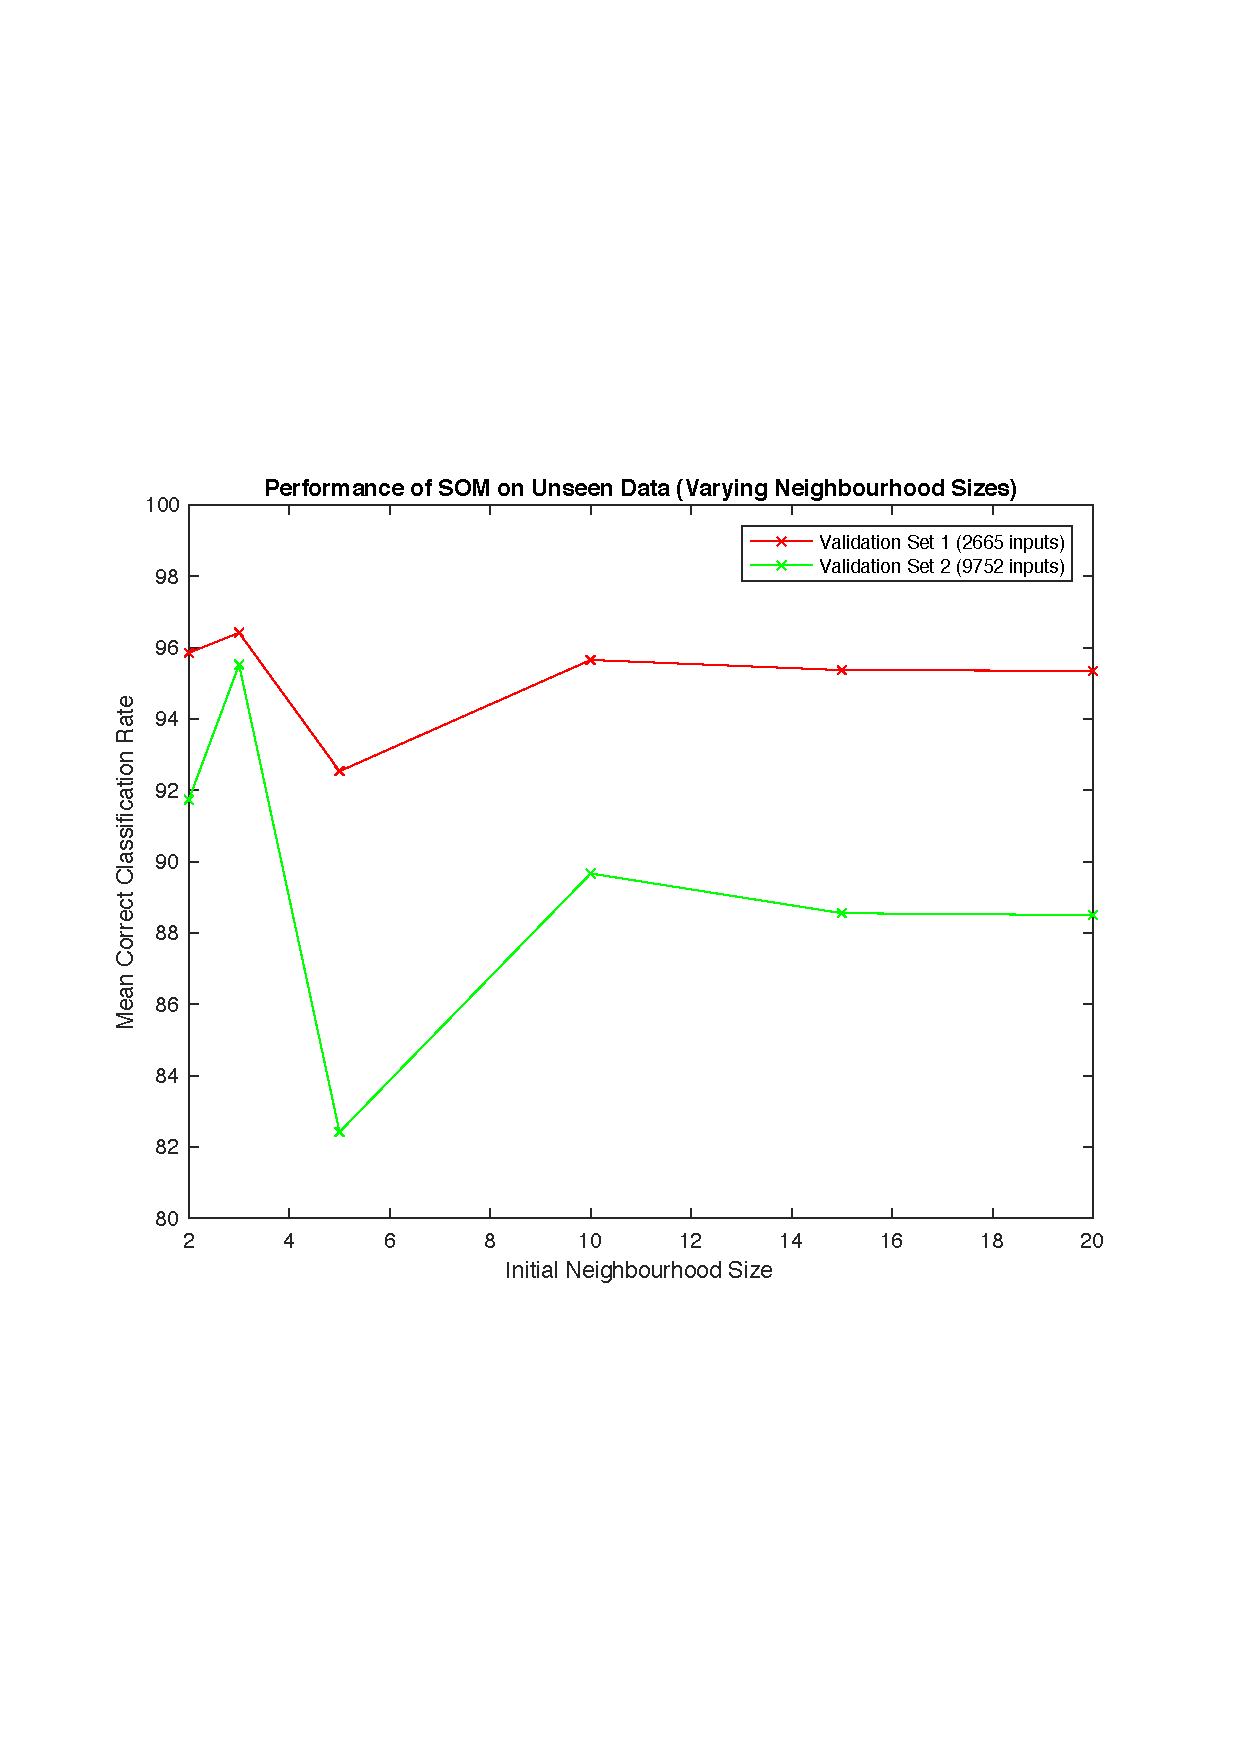
\includegraphics[width=7.5cm]{neighbourhood-plot.pdf}
\end{center}
\caption{\label{fig:testing-plots} Plots from testing varying number of training steps (left), varying neighbourhood sizes (right).}
\end{figure}

With number of steps at each phase of training set at 500, a few training configurations are tested at varying initial neighbourhood sizes at the default learning rate, as shown in Figure \ref{fig:neighbourhood-testing} and plotted in Figure \ref{fig:testing-plots} (right). The result is unanimous: the default initial neighbourhood size of 3 for the ordering phase produces the best results in both unseen validation datasets. The initial neighbourhood size for the convergence phase is set at 1.

\begin{figure}[h]
\begin{center}
\fontsize{9}{11}\selectfont
\begin{tabular}{|*{8}{c|}}
\hline 
Initial Neighbourhood Size & Data & 2 & 3 & 5 & 10 & 15 & 20 \\ \hline
\multirow{2}{*}{Training MSE} & Mean & 0.084 & 0.069 & 0.058 & 0.052 & 0.055 & 0.055 \\ \cline{2-8}
\ & Variance & \multicolumn{6}{c|}{$<$0.01} \\ \hline
\multirow{2}{*}{Validation 1 MSE} & Mean & 0.111 & 0.959 & 0.073 & 0.063 & 0.067 & 0.067 \\ \cline{2-8}
\ & Variance & \multicolumn{6}{c|}{$<$0.01} \\ \hline
\multirow{2}{*}{Misclassification 1 (\%)} & Mean & 4.15 & 3.58 & 7.46 & 4.35 & 4.63 & 4.65 \\ \cline{2-8}
\ & Variance & $<$0.01 & 0.072 & 0.002 & 0.136 & 0.154 & 0.132 \\ \hline
\multirow{2}{*}{Validation 2 MSE} & Mean & 0.165 & 0.125 & 0.142 & 0.126 & 0.137 & 0.138 \\ \cline{2-8}
\ & Variance & \multicolumn{6}{c|}{$<$0.01} \\ \hline
\multirow{2}{*}{Misclassification 2 (\%)} & Mean & 8.26 & 4.48 & 17.6 & 10.3 & 11.4 & 11.5 \\ \cline{2-8}
\ & Variance & 5.55 & 6.87 & $<$0.01 & 2.11 & 2.39 & 2.26 \\ \hline
\end{tabular}
\end{center}
\caption{\label{fig:neighbourhood-testing} Results from varying the number of steps in each phase of training on a [20 1] SOM.}
\end{figure}

Finally, the only two other adjustable parameters are the grid topology and distance function. As the experiments are conducted on a one-dimensional grid, the topology of the neurons will remain in a straight line no matter how the grid is organised, and have a consistent distance between any specific pair of neurons no matter the distance function. Therefore, the two parameters remain as hexagonal and linked distance. In summary, for the final training parameters, \textbf{the only change made to the toolbox defaults is the increase in number of steps in each phase of training} (from 100 to 500).

\subsection{Evaluations of Neural Networks}

\textbf{The final network}: In selecting the final network, with the training parameters determined in Section \ref{subsec:training}, the only variable to decide on is the size of the one-dimensional SOM. As the cursory test (Figure \ref{fig:som-testing}) has indicated a likely range of best performing SOM sizes, they are further tested on both validation datasets through ten fresh trainings with the determined training parameters, as shown in Figure \ref{fig:size-testing}.

\begin{figure}[h]
\begin{subfigure}{0.5\textwidth}
\fontsize{8}{10}\selectfont
\begin{tabular}{|p{2.0cm}|p{1.0cm}|p{0.7cm}|p{0.7cm}|p{0.7cm}|>{\bfseries}p{0.8cm}|p{0.7cm}|}
\hline 
SOM Size & Data & [10 1] & [20 1] & [30 1] & [40 1] & [50 1] \\ \hline
\multirow{2}{*}{\parbox{2.0cm}{\centering Training MSE}} & Mean & 0.040 & 0.066 & 0.081 & 0.062 & 0.080 \\ \cline{2-7}
\ & Variance & \multicolumn{5}{c|}{$<$0.01} \\ \hline
\multirow{2}{*}{\parbox{2.0cm}{\centering Validation 1 MSE}} & Mean & 0.053 & 0.092 & 0.108 & 0.077 & 0.103 \\ \cline{2-7}
\ & Variance & \multicolumn{5}{c|}{$<$0.01} \\ \hline
\multirow{2}{*}{\parbox{2.0cm}{\centering Misclassification 1 (\%)}} & Mean & 6.55 & 3.69 & 5.77 & 2.59 & 3.79 \\ \cline{2-7}
\ & Variance & $<$0.01 & 0.306 & 0.535 & 0.427 & 2.18 \\ \hline
\multirow{2}{*}{\parbox{2.0cm}{\centering Validation 2 MSE}} & Mean & 0.055 & 0.122 & 0.140 & 0.120 & 0.146 \\ \cline{2-7}
\ & Variance & \multicolumn{5}{c|}{$<$0.01} \\ \hline
\multirow{2}{*}{\parbox{2.0cm}{\centering Misclassification 2 (\%)}} & Mean & 7.59 & 4.87 & 4.35 & 3.65 & 8.88 \\ \cline{2-7}
\ & Variance & $<$0.01 & 12.5 & 0.214 & 0.074 & 16.5 \\ \hline
\end{tabular}
\end{subfigure}
\begin{subfigure}{0.5\textwidth}
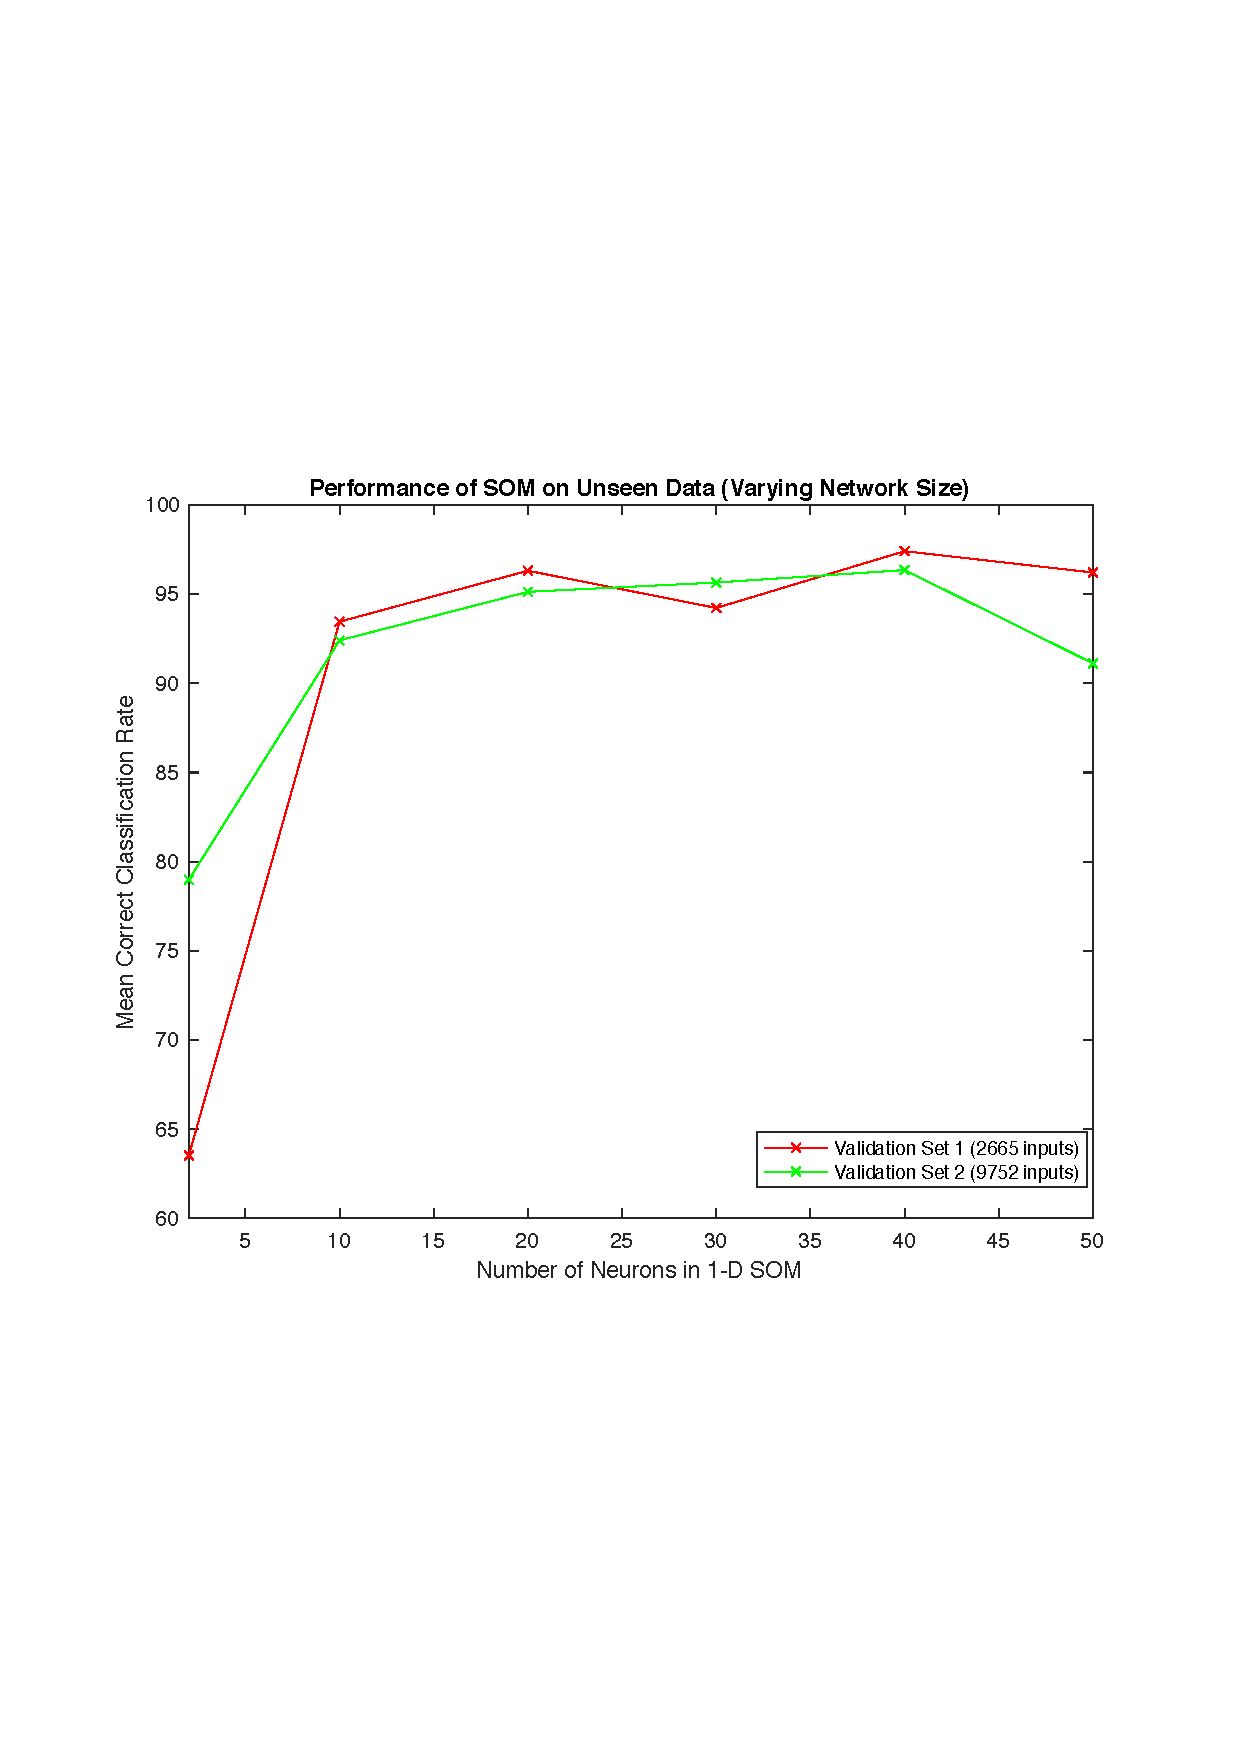
\includegraphics[width=7cm, right]{final-testing-plot.pdf}
\end{subfigure}
\caption{\label{fig:size-testing} Results from varying network size of the one-dimensional SOM.}
\end{figure}

It can be observed that while the [20 1] SOM used throughout the previous sections still performs very well, the performance of the larger [40 1] SOM is even better with the higher number of steps in each phase of training. With variances of 0.427 and 0.074 on the misclassification rate of unseen inputs across ten runs, there is good confidence that the [40 1] SOM is the best performing network size. Therefore, \textbf{the [40 1] SOM with the determined training parameters is selected as the final architecture and configuration}.

\textbf{The comparison metrics}: Because this problem is a binary (0/1) classification problem \cite[p. 28]{candanedo2016accurate}, the mean square error (MSE) of the network on either seen or unseen data is not a very meaningful measurement of performance (unless MSE gets very high, which implies the failure of the network). It may nevertheless be a good comparison between networks of the same type with different training parameters or sizes, therefore it has been included in all data figures in this report, alongside the misclassification rate. These two metrics have been used to evaluate and compare all architectures covered.

Due to the nature of the classification problem, it may be better to measure with the misclassification rate, which is defined as the fraction of a set of inputs that are placed on the half of SOM away from the cluster of that class of inputs. This is calculated based on an assumption described as followed.

As mentioned at the start of Section \ref{subsec:preprocessing}, an assumption was made that the one-dimensional SOM will cluster the two classes of inputs at the two ends of the map. During the course of this report, extensive observations on $plotsomhits$ have always showed that this is the case on one-dimensional SOMs without normalisation or PCA conducted on the input data. 

It was also observed that the positions of the two clusters have always been opposite to the ordering of the output vector (occupied/`1' inputs cluster on the low index end, unoccupied/`0' inputs cluster on the high index end). This is however, a projection of data in higher dimensions, and maybe arbitrary \cite[p. 10]{som-app-lecture}. While it appears that the toolbox implementation always projects the output data in this way, this is not a defined feature of the network.

Therefore, while it possible to infer the class of an input based on its position placed in the output vector from applying the SOM, the assumptions made here may be implementation specific (i.e. to the MATLAB toolbox). Some manual observations on the results of other implementations may be required before these assumptions can be carried over. 

\textbf{The architecture selection process}: Three architectures potentially suitable for the nature of input and target data were shortlisted based on my previous experience solving regression or classification problems with these architectures: the multi-layer perceptron (MLP), radial basis function (RBF) networks, and the self-organising map (SOM). The testing and selection process has been covered in detail in Section \ref{sec:architectures}. A number of possible training functions and/or network sizes were tested, and the MSE's and misclassification rates from these tests are the primary factors in determining the architecture of choice. Additional considerations were made regarding the easiness of implementation and long term retraining requirements, as the chosen architecture could be implemented in a commercial equipment for room occupancy detection purposes. 

While both MLP and SOM have shown similar superior performance over RBF, SOM was ultimately chosen to be evaluated and tested further, as its unsupervised training provides a unique benefit in reducing the maintenance requirement and increasing the adaptability of the network in fulfilling the specific purpose.

\textbf{Data used during selection}: During the architecture selection process, the data was divided in two datasets: the training dataset (8143 records), and the validation dataset (two testing datasets combined, 12417 records). The target data was used as is, while the input data had time removed, leaving five variables.

During the further testings of SOM, tests were conducted to determine the suitability of various pre-processing methods, as well as to choose the best training parameters. All further testings used the same training dataset and the two testing datasets separated (2665 and 9752 records), due to their distinct nature (the former recorded mostly with the door closed, and the latter mostly with the door opened \cite[Tb. 5]{candanedo2016accurate}). 

No further splitting of data was done, except the automatic splittings of dataset by MLP and RBF during the architecture selection. The toolbox implementation of SOM does not automatically preprocess data.

\subsection{Results of SOM testing}

The most prominent observation from the evaluations is that SOM can in fact produce very good results in binary classification through clustering features, with a possible extension to more variables. The performance of the final SOM on the unseen validation datasets yields a 2.59\% misclassification rate on the door-closed dataset, and 3.65\% on the door-open dataset, as shown in Figure \ref{fig:size-testing}. In comparison with the original research using different methods, which produced best misclassification rates of 2.1\% and 0.67\% on the two datasets \cite[p. 36]{candanedo2016accurate}, the SOM approach is not as good, although comparable to an average case reported by the research. 

Interestingly, the SOM approach consistently performs worse on the second, larger dataset across nearly all testings in this report. Without considering the contrary results from the original research, there seems to be a straightforward reason: data in the second dataset were collected under a different condition to the training dataset and the first validation dataset that -- the door is usually open for the second dataset. With the door open, the sensor data may exhibit small variations in their pattern, which should reduce but not improve the performance of the network. A possible explanation to this contradiction is that the actual occupancy level of the room is lower (64\%) in the first validation dataset than the other two datasets, which have a matching level of occupancy (79\%). While both the methods from the original research and neural networks such as MLP are in some way aware of this context change through supervised training on the training dataset, this is not the case for the unsupervised SOM, which may have posed it a disadvantage. This may have reduced SOM's performance when the sensor data patterns varied due to the door being left open, and it cannot compensate for this through context awareness. The SOM is also apparently unaffected by the inclusion of time or time sequence data (Figure \ref{fig:time-testing}), potentially for the same reason.

Nevertheless, the unsupervised training of SOM does allow an occupancy detection system to continuously and autonomously retrain to adapt to changes in long term data pattern, as no occupancy reference information is required for its continued retraining. 

Another interesting observation from the testing of SOM is that its classification performance increases as the network size increases until a peak level, then the performance decreases as more neurons are added. This is potentially due to the border effects of the SOM \cite[Sec. 4.5]{kohonen2014matlab} causing distortions at borders of neurons. An overly large number of neurons could accelerate this effect, making clustering-based classification less reliable.

Finally, choosing SOM for further evaluation in place of the more familiar MLP was not a decision taken lightly. During this report, I have attempted to apply conventional neural network approaches in data processing and experimentation, but some results were rather unexpected, such as the worsening effects both [0, 1] normalisation and PCA. However, based on SOM's overall performance in binary classification, I do believe that this application of SOM has a lot of potential for future exploration.

\section{Possible applications of neural networks in Building Management Systems (BMS)}

For Section B of the assessment, Section \ref{subset:mlp-additional} of this report discusses a potential use of MLP networks for humidity control in BMS, while Section \ref{subset:art-additional} discusses a potential use of ART networks for abnormality detection with BMS data.

\subsection{Automatic indoor humidity control with a multi-layer perceptron (MLP) network} \label{subset:mlp-additional}

For buildings located in climates with seasonal varying temperature levels, heating is usually required during Winter months. A forced-air heating system is often used for these buildings, on which a humidifier \cite{swimmer1970forced} usually needs to be attached to humidify the circulated air, prevent the air from becoming overly dry. However, as temperature and humidity of the system air intake change, the demand on the output of humidifier will change. It is necessary to maintain a suitable level of humidity by adjusting the output of the humidifier (and perhaps the heater itself), as humidity levels too high or too low can cause health problems and other damages \cite{humidity-factors}, as well as for energy saving reasons. In place of normal human monitoring, it may be possible for an automatic control system based on a multi-layer perceptron (MLP) network to take over.

\textbf{The network architecture}: A standard MLP network with backpropagation is to be implemented. The network will be divided into several layers, including an input layer, one or more hidden layers, and an output layer. The number of neurons on the input layer should match the number of inputs, while the number of neurons on a hidden layer as well as the number of hidden layers are to be determined through experimental training and evaluations. Neurons in the network are identical, each calculating a weighted sum of inputs with an activation function. The outputs from hidden layer neurons are then summed with weight by the output layer neuron to give a final output. \cite[p. 2]{rbf-lecture} This output could be scaled into a power level of the humidifier. A common training algorithm such as Levenberg-Marquardt could be used to train the MLP.

\textbf{The suitability of the architecture}: Depending on the equipment, the humidifier could simply have an on-off state operating at a fixed power level, or it could have an adjustable level of output. In the first case, the problem can simply be treated as a classification problem, which has been shown to be possible based on indoor sensor data with a relatively high level of accuracy in Section \ref{subsec:mlp-test} (while \ref{subsec:mlp-test} attempts to predict a condition of the room (occupancy), prediction of the on-off state of the humidifier can be done in the same way). In the second case, the problem requires a standard regression analysis, for which MLP has been shown to be useful in the context of BMS control \cite[Sec. 3.1]{kusiak2011multi}. With building sensor data coupled with machine operation records (possibly controlled by a human), a trained MLP should be able to automatically produce an operating state to control the humidifier similar to how a human would respond to changes in the room conditions.

\textbf{Data and training of the network}: Based on the recommendations of the government's Health and Safety Executive \cite{humidity-factors}, four environmental factors could affect the level of comfort: air temperature, radiant temperature from warm objects, air velocity and humidity. All four factors can be measured with environment sensors such as electronic temperature gauges, air velocity gauges and humidity meters. Several sensors of each type can be sparsely placed in the indoor environment to measure a median level of value (to reduce the effects of incidental extreme values on the input). In order to collect training data for the network, the humidifier can be operated by experienced human operators for a short period to time, with humidifier states recorded alongside sensor data. With preprocessed sensor data (imputation, PCA, etc.) as input and system states as target, the MLP can be trained to simulate how a human may operate the system under different conditions, hence be able to take control of the system from the human operator. 

\textbf{Responding to significant changes}: Despite trained on past sensor data and human operated humidifier states, the MLP may still produce inappropriate outputs for the conditions. This is particularly likely if a significant environmental change has occurred. Examples may include a particularly hot day in Spring, or the installation of a heavy equipment in the room. While the system may have the chance to identify and correct the error itself by monitoring the humidity meter based on a preset range of acceptable humidity levels, and retraining with new data if necessary, a human operator can also step in and correct the output, thus setting new targets for the MLP to retrain. This allows the BMS to remain well-adapted for the particular conditions of the indoor environment it operates in.

\subsection{Automatic abnormality detection with an Adaptive Resonance Theory (ART) network} \label{subset:art-additional}

Within an advanced BMS, electrical control of fixtures such as door locks and lights are connected with a central computing system. This provides the potential of adapting a pattern recognition-capable neural network for the purpose of automatic abnormality detection, such as detecting an intrusion to the property while the owners are away. The Adaptive Resonance Theory (ART) network has been identified with this potential.

\textbf{The network architecture}: The ART network is a fully-connected asymmetric-weight recurrent network, with two layers: an input/comparison layer and an output/recognition layer \cite[p. 7]{art-lecture}. The network is capable of autonomously managing pattern recognition and continued learning at the same time. The ART1 network accepts binary vectors only, while the ART2 variation can accept continuous inputs \cite[p. 21]{art-lecture}. Upon provided an input, the output from the network will reflect whether the pattern has been identified as a similar pattern to its existing long term memory, which will allow external systems to send the user a text message if an irregularity has been detected by the BMS. A vigilance threshold can be set by the user to adjust the sensitivity of the system \cite[p. 17]{art-lecture}.

\textbf{The suitability of the architecture}: The most prominent feature of the ART making it suitable for the use of long term abnormality detection is that it can manage its own continuous learning while simultaneously providing pattern recognition with existing knowledge. This allows the system to be installed with minimal training, after which it can adapt itself to suit the property it serves. Because different home users have very different activity routines, this feature could effectively reduce the number of false positives it detects. ART is also a stable network \cite[p. 5]{art-lecture}, allowing it to function consistently under regular patterns of use. While the ART1 network can only accept binary vectors, it is already sufficient to represent a wide range of BMS states, such as on/off status of lights in different rooms. With the continuous input support provided by ART2, more BMS states such as indoor noise level can be represented.

\textbf{Data and training of the network}: A very wide range of potential BMS states can be used as input, such as the on/off states of lights and other appliances, the times and frequencies of doors being opened, and the average noise levels as detected by indoor sensors. All these data can be useful in identifying the state of the property. For example, if on one day of the month the front door lock becomes disengaged at 3 am in the morning, it is plausible that this indicates an intrusion. The input data (both binary and continuous variables) will be stored in a vector and passed into an ART2 network for both pattern recognition and learning. The input then passes through the network, triggering a search for a matching pattern in the network. If a stored pattern is similar enough as determined by the configuration vigilance threshold, the new pattern is incorporated into that class of patterns in the memory, otherwise, the system reports an abnormality, and if it turns out to be a false positive, stores the pattern in a new class \cite[p. 18]{art-lecture}.

\textbf{Responding to significant changes}: As a live system, the patterns received by the ART may suddenly change but should not be considered an abnormality, such as when the occupiers of the property go on a vacation, keeping the lights off. Therefore, some false positives may be unavoidable until large enough number of new patterns eventually form a new long term memory trace in the network \cite[p. 7]{art-lecture}, when the new pattern is treated as familiar. To reduce the potential undue anxiety this may cause to a user away from their property, secondary systems can be used to inhibit certain types of alerts, such as a decrease of detected activity as opposed to an increase at certain times. While the ART itself usually cannot provide the nature of abnormality, this can be achieved by measuring BMS inputs mathematically in the secondary system. The secondary system can also be used to prevent consecutive alerts on the same mismatched pattern.

\bibliographystyle{IEEEtran}
\footnotesize{\bibliography{report}}
\end{document}  

